% Springer Nature / Machine Learning manuscript draft
% Compile in Overleaf with sn-jnl.cls in the project root.
% Recommended compiler: pdfLaTeX.
\documentclass[pdflatex,sn-mathphys-num]{sn-jnl}

\usepackage{graphicx}
% Look for figures both in a figures/ subfolder and in the project root,
% so \includegraphics resolves regardless of how the Overleaf project is organized.
\graphicspath{{figures/}{./}}
\usepackage{multirow}
\usepackage{amsmath,amssymb,amsfonts}
\usepackage{amsthm}
\usepackage{mathrsfs}
\usepackage[title]{appendix}
\usepackage{xcolor}
\usepackage{textcomp}
\usepackage{manyfoot}
\usepackage{booktabs}
\usepackage{tabularx}
\usepackage{array}
\usepackage{algorithm}
\usepackage{algorithmicx}
\usepackage{algpseudocode}
\usepackage{listings}

\raggedbottom
\sloppy
\emergencystretch=2em

%\jyear{2026}

\title[SENTINEL-SplitFed]{SENTINEL-SplitFed: Staleness-Aware Encoder Anomaly Detection for Intrusion-Resilient Asynchronous Split Federated Learning in Critical-Care Prediction}

\author*[1]{\fnm{Sumaiya Tabassum} \sur{Nimi}}\email{sumtamnimi@gmail.com}
\author[1]{\fnm{Tasbid Al} \sur{Rahman}}\email{tasbidrahman555@gmail.com}
\author[2]{\fnm{Hassin Arman} \sur{Nihal}}\email{hassinarman070@gmail.com}
\author[3]{\fnm{Md. Sorup} \sur{Rohan}}\email{sorupr5@gmail.com}

\affil*[1]{\orgdiv{Department of Electrical and Computer Engineering}, \orgname{North South University}, \orgaddress{\city{Dhaka}, \country{Bangladesh}}}
\affil[2]{\orgdiv{Department of Electrical and Electronic Engineering}, \orgname{Bangladesh University of Engineering and Technology}, \orgaddress{\city{Dhaka}, \country{Bangladesh}}}
\affil[3]{\orgdiv{Department of Computer Science and Engineering}, \orgname{Khulna University of Engineering \& Technology}, \orgaddress{\city{Khulna}, \country{Bangladesh}}}

\abstract{Split federated learning (SplitFed) pairs the label locality of split learning with federated aggregation, but existing pipelines assume synchronous aggregation and benign clients: the server waits for every client and accepts each submitted encoder without adversarial verification. Both assumptions are brittle in Internet of Medical Things deployments, where clients may be delayed and compromised clients may submit poisoned encoder weights. We propose SENTINEL-SplitFed, a server-side extension that replaces blocking aggregation with timed submission windows, tracks per-client staleness, and gates each submission by a Staleness-Normalized Anomaly Score (SNAS) combining cosine and norm encoder anomalies discounted by benign delay-induced staleness. On a three-client non-IID MIMIC-IV mortality benchmark, SNAS detects gradient-scaling, free-rider, label-flip and backdoor attacks in 100\% of post-warm-up attacker submissions (8/8; 80\% including the warm-up rounds, during which the gate is deliberately inactive), with no observed false positives (0/16 honest client-rounds) and no false quarantine of honest stragglers. Detection is not exclusion, however: direction-driven attacks score between the flag and quarantine thresholds, so the backdoor is flagged in every scored round yet remains the most damaging attack evaluated ($0.7008$ AUROC against a $0.9651$ clean baseline). SNAS outperforms trimmed mean and FLTrust on every attack setting, winning ten of ten paired seeds in each case (Wilcoxon $p=0.00195$, the $n=10$ floor). The coordinate-wise median, however, beats SNAS on both pure attacks by the same unanimous margin, and we report this rather than omit it. The ordering reverses only under straggling, where the median's breakdown point falls to zero in the $30\%$ of rounds that aggregate two clients. We therefore defend a narrower claim than aggregator dominance: quorum-dependent robustness degrades under asynchrony while per-submission detection does not. Krum's apparent advantage is a tie-break artifact of operating outside its own $N\geq2f+3$ condition and disappears at $N=6$, where its selection spreads across four honest clients and never names the adversary. Finally, an attack-then-abstain adversary evades memoryless staleness normalization -- a robustness boundary we characterize explicitly, showing it to be self-limiting, and for which we outline temporal accumulation as a mitigation direction.}

\keywords{split federated learning, asynchronous federated learning, Byzantine robustness, intrusion detection, critical-care machine learning, MIMIC-IV, IoMT}

\begin{document}

\maketitle

\section{Introduction}\label{sec:introduction}

Collaborative machine learning for healthcare must reconcile three competing requirements: predictive performance, institutional privacy, and operational robustness. In critical-care applications, patient cohorts are naturally distributed across hospitals, units, or edge devices; labels may be sensitive; and networked clients can differ substantially in compute capacity, connectivity, and workload. Federated learning (FL) addresses data locality by training a shared model across decentralized clients without directly pooling raw data \cite{mcmahan2017communication}. Split learning reduces client-side computation and can keep labels server-side or client-side depending on the protocol design \cite{vepakomma2018split}. Split federated learning (SplitFed) combines these ideas by splitting the model into a client-side encoder and a server-side top model while aggregating client encoders across participants \cite{thapa2022splitfed}.

Despite this promise, SplitFed systems face two practical limitations in critical-care deployments. First, aggregation is often synchronous: the server waits for all clients before updating the global encoder. This blocking design is poorly matched to IoMT settings in which devices, hospitals, or unit-specific clients may be delayed by network lag, compute heterogeneity, or patient-load variation. Second, many SplitFed pipelines trust registered clients at aggregation time. A compromised client can therefore submit malicious encoder weights, including random free-rider weights or gradient-scaled updates, without a native detection mechanism.

The core challenge is that benign staleness and malicious deviation can appear superficially similar. A slow client may submit an encoder that differs from the current global reference because it trained on an older model. A malicious client may submit an encoder that differs because it was adversarially modified. A detector based only on raw deviation risks falsely penalizing legitimate stragglers, while a detector that over-discounts staleness can be exploited by adaptive adversaries.

This paper presents \emph{SENTINEL-SplitFed}, an asynchronous split federated learning framework with intrusion resilience. The method is implemented as a server-side extension of a label-private SplitFed pipeline for MIMIC-IV mortality prediction. It introduces four mechanisms: (i) a timed asynchronous round controller that aggregates at window close rather than waiting for all clients (ii) a staleness registry that records consecutive missed rounds for each client (iii) a Staleness-Normalized Anomaly Score (SNAS) that combines cosine and norm anomalies of submitted encoders while normalizing by staleness and (iv) robust asynchronous aggregation with norm clipping and gate-based exclusion or downweighting.

The paper makes the following contributions.
\begin{itemize}
    \item We formulate intrusion-resilient asynchronous SplitFed for low-client critical-care federation, where the server must distinguish honest stragglers from malicious encoder submissions.
    \item We propose SNAS, a simple server-side anomaly gate that combines directional and magnitude-based encoder deviation and normalizes the score by client staleness.
    \item We evaluate SENTINEL-SplitFed on non-IID MIMIC-IV mortality prediction using honest straggler, gradient-scaling, free-rider, label-flip, backdoor, simultaneous attack-and-straggler, adaptive adversary, and hyperparameter sensitivity experiments. Separating detection from exclusion turns out to matter: the backdoor is flagged in every post-warm-up round yet scores below the quarantine threshold, and is consequently the most damaging attack we evaluate ($0.7008$ AUROC, $0.2459$ AUPRC). Direction-driven and magnitude-driven attacks occupy disjoint score ranges, so no single quarantine threshold serves both.
    \item We compare SNAS against Byzantine-robust FL baselines under matched conditions, and report the comparison in both directions. SNAS significantly outperforms trimmed mean and FLTrust on every attack setting, winning ten of ten paired seeds in each case; but the coordinate-wise median beats SNAS on both pure attacks, also ten of ten. The ordering reverses only when a client straggles, and the mechanism is measurable: robust aggregation rules earn their guarantee from a quorum of arrivals, so the median's breakdown point falls to zero in the $30\%$ of rounds that aggregate two clients, while per-submission detection is unaffected by arrival count. The claim we defend is therefore not that SNAS is the strongest robust aggregator, but that \emph{quorum-dependent robustness degrades under asynchrony while per-submission detection does not}.
    \item We quantify federation preservation with a contribution-entropy metric measured on the same runs: $H=0.000$ for Krum, which selects one client in every round, versus $H=0.986$ for SNAS in the clean setting and $H=0.249$--$0.767$ under attack, where the reduction reflects deliberate exclusion of the detected adversary. Repartitioning into six clients shows that Krum's collapse is an artifact of the $N=3$ regime violating its own $N\geq2f+3$ condition: at $N=6$ its selection spreads across four honest clients and never names the adversary, and its apparent accuracy advantage disappears.
    \item We ablate the anomaly gate against a no-detection asynchronous baseline (pure staleness-weighted FedAvg), showing that the gate recovers up to $0.097$ AUROC under attack while imposing no cost when clients are honest.
    \item We identify an important robustness boundary: memoryless staleness-normalized scoring can be evaded by an adversary that alternates between attacking and abstaining. We present this limitation as a concrete direction for temporal anomaly accumulation.
\end{itemize}

\section{Related Work}\label{sec:related}

Our work sits at the intersection of three research threads that have largely developed in isolation: asynchronous and straggler-resilient split federated learning, staleness-aware asynchronous federated learning, and Byzantine-robust aggregation. Existing asynchronous SplitFed methods mostly treat stragglers as an efficiency bottleneck, existing Byzantine-robust asynchronous FL methods mostly target malicious updates in standard full-model FL. SENTINEL-SplitFed targets the overlap that remains underexplored: in label-private SplitFed, the server must distinguish an honestly stale client encoder from a maliciously corrupted encoder before asynchronous aggregation.

\subsection{Federated and split learning}

Federated learning trains a global model from decentralized data by repeatedly aggregating client updates \cite{mcmahan2017communication}. In healthcare, FL is attractive because it avoids direct raw-data pooling, but standard FL can still expose full model updates and typically assumes that each client trains the same full model. Split learning partitions a neural network across client and server: the client computes activations up to a cut layer, the server completes the forward and backward pass, and gradients are returned to the client \cite{vepakomma2018split}. SplitFed combines split learning with federated aggregation of client-side model segments \cite{thapa2022splitfed}. The resulting design can reduce client computation and support label-private protocols, but introduces a new aggregation object: the client-side encoder, which is the unit our detector operates on. As classical architectures evolve, recent advancements are extending these paradigms into the quantum domain, introducing Quantum Federated Learning (QFL) to handle high-dimensional complex data over classical and quantum communication networks \cite{chehimi2024foundations}, and Quantum Split Learning (QSL) to integrate quantum neural networks for enhanced privacy protection and accelerated convergence \cite{yun2022quantum}.


\subsection{Asynchronous and straggler-resilient split federated learning}

The works closest to ours in architecture study asynchronous or straggler-resilient SplitFed, typically in healthcare or edge settings. Digital-twin-enabled asynchronous SplitFed for e-healthcare addresses resource heterogeneity, communication efficiency, and data privacy through digital-twin orchestration \cite{stephanie2023digital}. Adaptive asynchronous SplitFed for medical image segmentation adapts each client's learning rate and local epochs based on its training speed, dataset size, and packet-loss probability \cite{shiranthika2024adaptive}. Privacy-preserving asynchronous SplitFed for smart healthcare combines weight-based aggregation with secure aggregation to accommodate heterogeneous device speed \cite{app2024splitfed}. MU-SplitFed decouples training progress from straggler delays via an unbalanced update mechanism, allowing the server to perform multiple local updates per client round \cite{liang2025straggler}. Foundational Asynchronous Federated Split Learning (AFSL) architectures demonstrate that allowing edge servers to independently update weights without waiting for stragglers can accelerate learning by up to 86\% while minimizing resource consumption for constrained edge devices \cite{albuquerque2024asynchronous}. Recent state-of-the-art approaches, such as Generative Activation-Aided Asynchronous SFL (GAS), address the bias introduced by these asynchronous transmissions by using activation and model buffers to manage delayed client updates \cite{yang2025gas}. The central goal of these methods is operational efficiency: reducing waiting time, adapting to heterogeneous client speeds, or mitigating straggler-induced update bias. SENTINEL-SplitFed differs by making the straggler itself part of the security problem: a late encoder is not merely a scheduling inconvenience, because it can be confused with a poisoned encoder unless the server explicitly models both staleness and anomaly.

\subsection{Staleness-aware asynchronous federated learning}

Synchronous FL waits for a fixed set of clients before aggregation, which creates a straggler bottleneck. Asynchronous FL relaxes this by updating from partial or delayed submissions, usually with staleness-aware weighting. FedAsync weights each stale update by a function of its staleness \cite{xie2019asynchronous}, and FedBuff aggregates buffered asynchronous updates to improve stability and efficiency \cite{nguyen2022fedbuff}. These methods motivate the need to model staleness explicitly, but they generally operate on full-model or gradient updates and do not address the split-learning case in which the server aggregates client encoders while simultaneously managing activation--gradient exchange. Crucially, convergence analyses of SFL show that client-side aggregation frequency directly shapes learning performance, so aggregation timing cannot be altered for free \cite{adaptsfl2025}. SENTINEL-SplitFed borrows the intuition that staleness must be modeled, but introduces a security use of staleness: normalizing anomaly scores so that benign delay is not automatically treated as malicious deviation.

\subsection{Byzantine-robust and secure asynchronous aggregation}

Byzantine-robust FL methods tolerate malicious or corrupted client updates. Krum selects the update closest to its neighbors in weight space \cite{blanchard2017machine}. Coordinate-wise median and trimmed mean reduce the influence of extreme coordinate values \cite{yin2018byzantine}. FLTrust uses a clean server root dataset to compute a trusted reference gradient and reweights client updates by cosine similarity with that reference \cite{cao2021fltrust}. More recent work extends robustness to the asynchronous setting: AFLGuard bridges Byzantine robustness and asynchronous FL using a server-side reference update \cite{fang2022aflguard}. Specifically, AFLGuard handles the noise inevitably introduced by client delays by equipping the central server with a small, clean trusted dataset. When evaluating an asynchronous submission, the server rejects the client's model update if it deviates substantially from the server's trusted model update with respect to direction and/or magnitude. Recent 2026 frameworks, such as Belisa, further extend this reference-based paradigm by quantifying discrepancies between feature representations (feature fingerprints) to cluster and filter malicious models under high data heterogeneity \cite{peng2026belisa}. AsyncDefender similarly targets Byzantine robustness under fully asynchronous participation, but avoids a fixed trusted reference set: it dynamically adjusts per-client trust and aggregation weight from the cosine similarity between each client update and the current global model, without assuming an upper bound on the number of malicious clients \cite{asyncdefender2025}.

These methods are important baselines and stronger references for standard asynchronous FL security, but they are not designed around SplitFed encoder aggregation, low-client cross-silo healthcare settings, or the distinction between missed activation windows and malicious encoder submissions. Moreover, low-client split learning exposes failure modes that are less visible in standard FL: Krum may repeatedly select a single client and collapse federation, trimmed mean may become vanilla averaging when the number of clients is small, and FLTrust requires a server-side reference gradient for the same parameter block being aggregated --- which in the split architecture can be obtained only by backpropagating a server-held root batch through the server head into the encoder, and only from a retained previous-round encoder. Section~\ref{sec:results} shows that this adaptation is feasible and that FLTrust is a functioning baseline once it is made, but also that an implementation lacking either half degenerates silently to uniform averaging while still reporting itself as FLTrust. We therefore position SENTINEL-SplitFed not as a universal replacement for these methods but as an architecturally specific mechanism for the SplitFed encoder-aggregation setting.

\subsection{Vertical split learning and SplitFed security}

A separate line of work studies straggler resilience and privacy in vertical split learning. FedVS designs secret-sharing schemes for local data and models so that the aggregate of client embeddings is reconstructed losslessly from non-straggling clients, guaranteeing information-theoretic privacy against colluding clients and a curious server \cite{li2023fedvs}. While early works like FedVS focus on honest-but-curious threat models, recent research has revealed severe vulnerabilities in both standard Split Learning and SplitFed architectures against active malicious participants. For instance, comprehensive vulnerability analyses demonstrate that distance-based and untargeted data poisoning attacks can severely degrade classifier outcomes in SFL environments \cite{alferaidi2025analyzing}. To counter these threats in standard split learning, defenses such as SafeSplit employ circular backward analysis and rollback mechanisms to detect client-side backdoors \cite{safesplit2025}, while SecureSplit utilizes dimensionality transformation and majority-based voting to separate and filter poisoned embeddings \cite{dou2026securesplit}. Furthermore, the emergence of stealthy targeted poisoning attacks (TPA-VSL) emphasizes that vertical split learning is highly susceptible to instance-specific embedding model manipulation without relying on traditional test-time triggers \cite{tpavsl2026}. These evolving adversarial landscapes confirm that SplitFed exhibits entirely different robustness and privacy behaviors compared to standard FL. We build on this observation by proposing SENTINEL-SplitFed, implementing an explicit server-side intrusion gate for the encoder block, moving beyond merely measuring vulnerability to actively neutralizing staleness-aware encoder poisoning.

\subsection{Critical-care prediction with MIMIC-IV}
MIMIC-IV is a widely used critical-care database containing de-identified ICU data \cite{johnson2023mimic}. Mortality prediction from MIMIC-IV is a useful stress test for collaborative healthcare learning because the data are heterogeneous across clinical units and the outcome is clinically important. Recent 2025 studies have increasingly adopted MIMIC-IV to validate decentralized predictive models, demonstrating that federated learning approaches can achieve mortality prediction accuracies comparable to centralized machine learning while ensuring stringent data privacy \cite{healthinf25}. However, comprehensive framework analyses reveal that while Split-FL architectures provide the highest level of privacy for multi-disease prediction on MIMIC-IV, they inherently suffer from severe communication and computational overheads \cite{cryptenfl2025}. This trade-off underscores the necessity of optimizing collaborative architectures. In this work, MIMIC-IV clients correspond to non-IID ICU partitions, allowing the evaluation to combine predictive performance, client heterogeneity, asynchronous participation, and adversarial aggregation, while actively mitigating the systemic overheads identified in modern secure healthcare FL deployments.

\subsection{Positioning}

In summary, the intersection of asynchronous execution and adversarial robustness within split federated learning exposes a critical multi-dimensional research gap. Existing asynchronous SplitFed architectures (such as AFSL and GAS) focus strictly on system efficiency and straggler latency mitigation, completely omitting active defense layers against compromised participants. Conversely, state-of-the-art asynchronous Byzantine defenses (such as AFLGuard and feature fingerprinting frameworks) are designed around standard, full-model federated learning pipelines. We do not claim these are inapplicable to SplitFed: Section~\ref{sec:results} demonstrates the opposite by adapting FLTrust to the encoder block and running it as a functioning baseline. The gap is narrower and more specific. First, the adaptation is non-obvious and silently failure-prone --- a reference gradient must be routed through the server head into the encoder and taken from a retained previous-round model, and an implementation missing either half degenerates to uniform averaging without error. Second, and more fundamentally, these defenses derive their guarantee from a quorum of concurrently arriving submissions: Krum needs $N\geq2f+3$ present, trimmed mean needs enough values to trim, and peer-referenced trust needs peers. Asynchronous participation makes partial arrival routine, and Section~\ref{sec:results} measures the consequence directly --- the coordinate median, the strongest baseline here under full participation, loses its Byzantine tolerance entirely in the $30\%$ of rounds where only two clients arrive. None of these methods models client staleness at all, so none can separate an honestly late encoder from a poisoned one. Furthermore, while emerging quantum-enhanced distributed paradigms (QFL and QSL) and localized embedding filters (such as SafeSplit) lay vital blueprints for future secure topographies, they do not yet address the temporal overlap where honest, networking-induced staleness mimics active encoder poisoning anomalies. 

\emph{SENTINEL-SplitFed} addresses this gap. It targets an underexplored intersection: an asynchronous, horizontal SplitFed architecture that jointly handles benign stragglers and malicious encoder submissions via a low-overhead, server-side decision rule that scores each submission against an anchor rather than against its peers, and is therefore unaffected by how many clients arrived. Rather than claiming dominance over generalized, massive-scale Byzantine-robust FL, we establish a defense specific to low-client, label-private, critical-care split-learning federations, and we report the settings in which correctly configured robust aggregators match or exceed it. Table~\ref{tab:sota-positioning} summarizes this positioning against representative FL and SplitFed robustness methods.

\section{Problem Setting and Threat Model}\label{sec:problem}

\subsection{SplitFed setting}

We consider $N$ clients indexed by $i\in\{1,\ldots,N\}$ and a central server. Each client owns a local dataset $\mathcal{D}_i$ and a client-side encoder $f_{\theta_i}$. The server owns a top model $g_\phi$. For an input batch $x_i$, client $i$ computes an activation
\begin{equation}
    a_i = f_{\theta_i}(x_i),
\end{equation}
and sends $a_i$ to the server. The server computes predictions $\hat{y}_i = g_\phi(a_i)$ and returns the raw logits to the client. The client evaluates the supervised loss against its locally held label and backpropagates to obtain $\partial \mathcal{L}/\partial \hat{y}_i$, which it sends back to the server; the server backpropagates through $g_\phi$ to obtain $\partial \mathcal{L}/\partial a_i$ and returns it to the client, which updates $\theta_i$ locally. Labels never leave the client. At aggregation time, clients submit encoder parameters $\theta_i$ to the server, and the server produces a global encoder $\theta^g$ for redistribution.

The framework is label-private in the operational sense that the split protocol does not require clients to transmit raw labels with encoder submissions. It does not claim cryptographic privacy for activations, gradients, or model updates. Differential privacy, secure aggregation, and activation perturbation are complementary mechanisms outside the present scope.

\subsection{Asynchronous participation}

Each aggregation round $r$ opens a submission window. A client may submit within the window, submit late, or miss the round. Synchronous aggregation waits for all clients, while SENTINEL-SplitFed aggregates using the submissions available at window close. For each client, the server tracks a staleness counter $\tau_i(r)$ defined as the number of consecutive rounds before round $r$ in which client $i$ did not contribute to aggregation.

\subsection{Threat model}

We assume the server can authenticate registered clients but cannot assume that every registered client is honest. A malicious client can modify the encoder submitted at aggregation time. We evaluate the following attacks.
\begin{itemize}
    \item \textbf{Gradient scaling:} the attacker multiplies all encoder tensors by a scalar, e.g., $10\times$, preserving direction while inflating magnitude.
    \item \textbf{Free rider:} the attacker submits random encoder weights and contributes no useful learned signal.
    \item \textbf{Attack plus straggler:} one client is malicious and on time, while another client is honestly delayed and repeatedly misses the window.
    \item \textbf{Adaptive threshold-aware attack:} the attacker knows the SNAS formula and attempts to choose a scale that remains below quarantine.
    \item \textbf{Strategic alternation:} the attacker alternates between attacking and abstaining to exploit staleness normalization.
    \item \textbf{Slow-ramp mimicry:} the attacker gradually increases the scale factor over rounds.
\end{itemize}

The goal is not to provide cryptographic Byzantine security. Instead, the goal is to design and empirically characterize a detection and aggregation mechanism that operates on the SplitFed aggregation object --- the client-side encoder --- and resists realistic encoder-submission attacks while avoiding false quarantine of benign stragglers.

We are precise about where the split-learning specificity of this contribution lies, since it bears on how the novelty should be assessed. The two anomaly signals themselves, cosine and norm deviation of submitted parameters, are architecture-agnostic and could be computed in any federated setting. What is specific to SplitFed is the object they are computed on and the information the server has available: the server holds only the encoder and the top model, never a full client network, so it cannot validate a submission against a locally reproducible reference model in the way a standard FL server can. This is the same constraint that requires FLTrust's reference gradient to be routed through the server head rather than computed directly (Section~\ref{sec:results}), and it is why staleness-aware gating is applied at the encoder-aggregation boundary. A third, genuinely split-learning-specific signal is available in principle --- divergence of the transmitted activations, which exist only because SplitFed sends them --- and our implementation computes it, but we set its weight to zero throughout because it did not discriminate the attacks evaluated here. We therefore claim the contribution at the level of the aggregation object and the asynchronous decision the server must make, not at the level of the anomaly statistics.

The scope is deliberately limited to attacks on the encoder parameters $\theta_i$ submitted at aggregation time. Poisoning of the server-side top model $g_\phi$ during split training --- for example, a client that returns manipulated logit gradients during the forward/backward exchange in order to corrupt $g_\phi$ --- is \emph{out of scope and not defended} by SNAS. In every experiment reported here, the malicious client trains honestly through the split protocol and perturbs only the encoder state it submits for aggregation, so $g_\phi$ is never poisoned. A defense for the server head would require a separate mechanism, such as gradient-level validation on a server-held reference batch or checkpoint rollback; we identify this as future work in Section~\ref{sec:limitations}.

\section{SENTINEL-SplitFed}\label{sec:method}

\subsection{Overview}

SENTINEL-SplitFed inserts four modules between the client encoder submission endpoint and the aggregation logic: an asynchronous round controller, a staleness registry, the SNAS detection gate, and robust asynchronous aggregation. The client-side split-learning protocol remains unchanged. The four are described in turn below and composed into a single server round in Algorithm~\ref{alg:server}.

\subsection{Asynchronous round controller}

At the beginning of round $r$, the server opens a submission window of duration
\begin{equation}
    T_{\mathrm{adaptive}}(r) = T_{\mathrm{base}}\left(1 + 0.1\cdot \frac{1}{N}\sum_{i=1}^{N}\tau_i(r)\right).
\end{equation}
The default local simulation uses $T_{\mathrm{base}}=25$ seconds. The adaptive factor slightly expands the window when the system observes persistent staleness. Aggregation proceeds when the deadline is reached, regardless of how many clients submitted.

\subsection{Staleness registry}

For each client, the server maintains
\begin{equation}
\tau_i(r) = \#\{\text{consecutive rounds before }r\text{ in which client }i\text{ missed aggregation}\}.
\end{equation}
The counter resets to zero when the client contributes within the window and increments by one when the client misses. The staleness value is used both in SNAS and in aggregation weighting.

We state explicitly what this counter does and does not measure, because the distinction bounds several of the results that follow. $\tau_i$ records \emph{missed participation}: how many consecutive aggregations a client was absent from. It is not a measure of model-version divergence. In this implementation every client fetches the current global encoder at the start of each round, including a client that missed the preceding round, so a client with $\tau_i>0$ still trains from the newest available model and its submission is not stale in the parameter sense. The two quantities coincide only when a client trains from the version it last fetched. A version-based formulation, $\tau_i(r)=r-v_i$ where $v_i$ is the last global version the client actually pulled, would require the client loop to retain the fetched encoder across a missed round and is left to future work. Two consequences follow, and we flag them where they arise: the honest-straggler result in Section~\ref{sec:results} shows that delayed \emph{participation} alone does not degrade accuracy, which is a weaker statement than showing that stale \emph{model versions} do not; and in the attack-then-abstain analysis of Section~\ref{sec:discussion} an abstaining adversary forfeits aggregation weight but does not additionally suffer from training on an outdated encoder.

We implement four decay functions for aggregation:
\begin{align}
    d_{\mathrm{linear}}(\tau) &= \frac{1}{1+\alpha\tau}, \\
    d_{\mathrm{exp}}(\tau) &= \exp(-\alpha\tau), \\
    d_{\mathrm{poly}}(\tau) &= \frac{1}{1+\tau^\kappa}, \\
    d_{\mathrm{step}}(\tau) &= \mathbb{I}[\tau \leq c_{\mathrm{step}}].
\end{align}
The default is exponential decay with $\alpha=0.5$.

\subsection{Staleness-Normalized Anomaly Score}

SNAS compares a submitted encoder $\theta_i$ against the previous global encoder $\theta^g$. Let $K$ denote the number of parameter tensors. The cosine anomaly is
\begin{equation}
    A^{\mathrm{cos}}_i = 1 - \frac{1}{K}\sum_{k=1}^{K}\cos\left(\mathrm{vec}(\theta_{i,k}),\mathrm{vec}(\theta^g_{k})\right).
\end{equation}
This detects directional deviations but is insensitive to scaling. Therefore, SNAS also computes a norm anomaly,
\begin{equation}
    A^{\mathrm{norm}}_i = \frac{1}{K}\sum_{k=1}^{K}\min\left(\frac{\left|\log\left(\frac{\|\theta_{i,k}\|_2}{\|\theta^g_k\|_2+\epsilon}\right)\right|}{\log(100)},1\right),
\end{equation}
where the cap corresponds to a $100\times$ norm ratio. The final score is
\begin{equation}
    \mathrm{SNAS}_i(r)=\frac{\beta A^{\mathrm{cos}}_i + \gamma A^{\mathrm{norm}}_i}{1+\tau_i(r)}.
\end{equation}
We use $\beta=0.35$ and $\gamma=0.65$ by default. The denominator discounts anomaly scores for stale clients, reducing false positives on benign delayed updates. The numerator remains high for strong weight-space attacks, especially when $\tau_i=0$.

The gate is held inactive for the first two aggregation rounds (rounds 1 and 2), and all submissions in that period are accepted regardless of score. Two rounds are required rather than one: no global encoder exists before the first aggregation, so no reference is available for either weight anomaly, and immediately after that aggregation each client's rolling reference has been updated exactly once and has not yet stabilized. With ten rounds per run this leaves eight scored rounds per client, which is the denominator used for all detection and false-positive rates reported in Section~\ref{sec:results}. After warm-up, each submitted client receives one of three gate decisions:
\begin{equation}
    \mathrm{gate}_i=\begin{cases}
        \mathrm{accept}, & \mathrm{SNAS}_i\leq \delta_{\mathrm{flag}},\\
        \mathrm{flag}, & \delta_{\mathrm{flag}} < \mathrm{SNAS}_i\leq \delta_{\mathrm{quarantine}},\\
        \mathrm{quarantine}, & \mathrm{SNAS}_i > \delta_{\mathrm{quarantine}}.
    \end{cases}
\end{equation}
The default thresholds are $\delta_{\mathrm{flag}}=0.22$ and $\delta_{\mathrm{quarantine}}=0.35$. Flagged clients are included with an aggregation penalty. Quarantine is a persistent state rather than a per-round decision: a quarantined client is excluded from aggregation and remains excluded until it has produced $K_{\mathrm{rehab}}=3$ consecutive submissions that score in the accept band, at which point it is rehabilitated and re-enters the aggregate. A single clean submission is therefore not sufficient to re-admit a client, and any flagged or quarantined submission in the interim resets the counter. This is what allows an attacker that intermittently scores below threshold to be held out across rounds in which it would individually have been accepted. These values were fixed on a calibration set consisting of the clean runs and the gradient-scaling attack only; every detection and false-positive rate reported in Section~\ref{sec:results} for the remaining attacks is measured on data that had no influence on them. Section~\ref{sec:calibration} states the procedure and the held-out result.
\begin{table}[htbp]
\caption{Positioning SENTINEL-SplitFed against representative FL and SplitFed robustness methods.}
\label{tab:sota-positioning}
\centering
\scriptsize
\setlength{\tabcolsep}{3pt}
\renewcommand{\arraystretch}{1.18}
\begin{tabularx}{\textwidth}{@{}p{2.05cm}p{2.25cm}ccc>{\raggedright\arraybackslash}X@{}}
\toprule
Method & Main goal & Async & Robust & SplitFed & Behavior in our setting \\
\midrule

FedAvg / SplitFed
& Collaborative decentralized training
& No
& No
& Partial
& Strong clean AUROC, but blocks on stragglers and accepts poisoned encoders. \\

FedAsync / FedBuff
& Reduce straggler delay
& Yes
& Limited
& No
& Useful for timing, but not designed to detect malicious SplitFed encoder submissions. \\

Krum
& Byzantine client selection
& No
& Yes
& No
& At $N=3$ higher raw AUROC, but selects one client every round, collapsing federation --- a tie-break artifact of violating $N\geq2f+3$. Resolves at $N=6$ (Section~\ref{sec:n6}). \\

Trimmed mean
& Coordinate-wise robust aggregation
& No
& Yes
& No
& Degenerates at three clients: with trim ratio 0.2, $\lfloor0.2\times3\rfloor=0$ values are trimmed and the rule is the unweighted mean. Valid at $N=6$. \\

Coordinate median
& Coordinate-wise robust aggregation
& No
& Yes
& No
& Strongest baseline under full participation, beating SNAS on both pure attacks; but at two arrivals the median \emph{is} the mean, so its tolerance vanishes when a client straggles. \\

FLTrust
& Trust-weighted FL using a root gradient
& No
& Yes
& No
& Functions once adapted to SplitFed --- reference gradient taken from the previous round's encoder, trust computed over updates --- but degenerates silently to uniform averaging without both adaptations. \\

Temporal poisoning detectors
& Detect inconsistent update trajectories
& Limited
& Yes
& No
& Motivate temporal SNAS accumulation, but are not directly designed for SplitFed encoder aggregation. \\

\textbf{SENTINEL-SplitFed}
& Intrusion-resilient asynchronous SplitFed
& \textbf{Yes}
& \textbf{Yes}
& \textbf{Yes}
& Preserves federation, detects all four non-adaptive attacks (gradient scaling, free rider, label flip, backdoor), and is the only rule here whose guarantee does not depend on how many clients arrived. But it quarantines only the norm-driven ones, so the backdoor still does damage while flagged, and it remains vulnerable to attack-then-abstain alternation. \\

\bottomrule
\end{tabularx}
\end{table}
\subsection{Robust asynchronous aggregation}\label{sec:agg}

For each non-quarantined submission, the raw aggregation weight is
\begin{equation}
    \omega_i = n_i \cdot d(\tau_i)\cdot p_i,
\end{equation}
where $n_i$ is the client training set size, $d(\tau_i)$ is the staleness decay, and $p_i=0.5$ for flagged clients and $p_i=1.0$ for accepted clients. The weights are normalized as $\bar{\omega}_i = \omega_i/\sum_j\omega_j$, and the global encoder is updated by
\begin{equation}
    \theta^g \leftarrow \sum_{i\in\mathcal{S}_r}\bar{\omega}_i\theta_i,
\end{equation}
where $\mathcal{S}_r$ is the set of accepted or flagged submissions in round $r$.

Before aggregation, each submitted tensor is clipped relative to the previous global tensor:
\begin{equation}
    \theta_{i,k}\leftarrow \theta_{i,k}\cdot \min\left(1,\frac{c_{\mathrm{clip}}\|\theta^g_k\|_2}{\|\theta_{i,k}\|_2+\epsilon}\right),
\end{equation}
with default $c_{\mathrm{clip}}=2.0$. If all submitted clients are quarantined, aggregation is skipped and the previous global encoder is retained.

\begin{algorithm}[htbp]
\caption{SENTINEL-SplitFed server round}
\label{alg:server}
\begin{algorithmic}[1]
\State Open asynchronous submission window for round $r$
\State Collect encoder submissions until $T_{\mathrm{adaptive}}(r)$ expires
\For{each registered client $i$}
    \If{$i$ submitted within the window}
        \State Compute $A^{\mathrm{cos}}_i$, $A^{\mathrm{norm}}_i$, and $\mathrm{SNAS}_i$ using arrival staleness $\tau_i$
        \State Assign gate decision: accept, flag, or quarantine
    \EndIf
\EndFor
\State Clip non-quarantined submitted tensors using $c_{\mathrm{clip}}$
\State Aggregate accepted and flagged encoders using staleness-decayed weights (staleness $\tau_i$ as of arrival)
\State Distribute the updated global encoder
\For{each registered client $i$}
    \If{$i$ submitted within the window}
        \State Reset $\tau_i\leftarrow0$
    \Else
        \State Mark missed round and set $\tau_i\leftarrow \tau_i+1$
    \EndIf
\EndFor
\end{algorithmic}
\end{algorithm}

\section{Experimental Setup}\label{sec:setup}

\subsection{Dataset and clients}

We evaluate on MIMIC-IV v3.1 \cite{johnson2023mimic}. The role of this benchmark in the present study should be stated plainly: it is a \emph{substrate for the security evaluation}, not a clinical mortality model. All comparisons in Section~\ref{sec:results} --- SNAS against Krum, trimmed mean, FLTrust, and the no-detection ablation --- are relative comparisons conducted on an identical data pipeline, so the security conclusions do not depend on the absolute predictive number. We do not claim clinical deployability, and Section~\ref{sec:limitations} states the specific reasons why the absolute AUROC reported here should not be compared against the published MIMIC-IV mortality literature.

\paragraph{Cohort and label.} One row is one ICU stay (\texttt{stay\_id}), obtained by joining \texttt{icustays} to \texttt{admissions} on \texttt{hadm\_id} and to \texttt{patients} on \texttt{subject\_id}. The prediction target is in-hospital mortality, taken directly from the admission-level \texttt{hospital\_expire\_flag}. No length-of-stay, readmission, or post-discharge filtering is applied.

\paragraph{Features and aggregation scope.} Each stay is described by 265 numeric features in five groups: 168 laboratory features (24 analytes $\times$ \{mean, min, max, std, measurement count, abnormal-flag count, STAT-order count\}), 84 vital-sign features (14 signals $\times$ \{mean, min, max, std, measurement count, warning count\}), 3 urine-output features, 5 binary vasopressor-administration indicators, and 5 demographic and administrative features (age, and encoded gender, insurance, race, and admission type).

Two properties of this aggregation must be stated explicitly, because they bound what the benchmark can support. First, \textbf{there is no observation window}: laboratory values are aggregated over the \emph{entire hospital admission} and vital signs over the \emph{entire ICU stay}, rather than over a fixed early window such as the first 24 hours that is standard in the clinical prediction literature. Because the label is whole-admission mortality, the feature window for a non-survivor therefore extends through terminal deterioration up to the time of death. Second, \textbf{the train/validation split is at row level, not patient or admission level}: laboratory features are joined at \texttt{hadm\_id} while rows are ICU stays, so an admission comprising multiple ICU stays contributes several rows carrying an identical laboratory block and an identical label, and the stratified 80/20 split may place such rows on both sides. Both properties inflate the absolute AUROC relative to a windowed, group-split benchmark. They apply identically to every aggregator compared here.

To remove the most direct source of label leakage, length of stay (\texttt{los}) is \textbf{excluded} from the feature set. Length of stay is only known at discharge and is strongly coupled to in-hospital death, so its presence as an input would leak the target; excluding it reduces the feature count from 266 to 265.

\paragraph{Imputation and scaling.} Missing aggregates --- arising when an analyte or signal was never recorded for a stay --- are filled with zero. Continuous features are standardized with a \texttt{StandardScaler} fitted \emph{on the training partition only} and then clipped to $[-5,5]$ to bound outliers such as very large measurement counts; the 5 binary vasopressor indicators are passed through unscaled. Scalers are fitted per client and never shared, consistent with the federated setting.

\paragraph{Client partition.} The benchmark is partitioned into three non-IID clients by ICU care unit, giving the natural clinical heterogeneity of a low-client hospital federation: Medical ICU (36{,}152 stays, 16.1\% mortality), Surgical ICU (23{,}483 stays, 11.5\%), and Cardiac ICU (32{,}743 stays, 6.9\%). Prevalence therefore spans a factor of $2.3$ across clients, which is the intended non-IID stress on aggregation.

\paragraph{Architecture and schedule.} The client encoder maps the 265 input features to a 32-dimensional representation through a hidden layer of size 64. The server top model maps the 32-dimensional activation to a binary mortality prediction through a hidden layer of size 64. Unless otherwise stated, experiments use 200 batches per client per round, batch size 64, and 10 aggregation rounds. Aggregation rounds are numbered from one throughout this paper, matching Figure~\ref{fig:perround}; the gate is inactive in rounds 1 and 2 and scores every submission from round 3 onward.

\paragraph{Execution model, and what ``asynchronous'' means here.} All experiments run against a single server process on one machine, with the clients executed sequentially within one driver process and their configured arrival offsets realized as explicit waits rather than as genuine network or compute latency. The asynchrony under evaluation is therefore \emph{windowed}, or buffered: the server aggregates whatever has arrived when the window closes instead of blocking until every client reports, and clients whose offset exceeds the window are absent from that aggregation. This reproduces the decision the server must make under partial participation, which is what SNAS operates on, and it makes the arrival pattern exactly reproducible across seeds and aggregators --- a requirement for the paired comparisons used throughout Section~\ref{sec:results}. It does not reproduce concurrent execution, so we report no wall-clock, time-to-target-AUROC, or per-round waiting metrics: with sequential clients no such speedup exists to measure, and any figure we quoted would be an artifact of the harness rather than a property of the method. Establishing the throughput benefit of asynchronous SplitFed requires a genuinely distributed deployment and is outside the scope of this evaluation.

\subsection{Metrics}

The primary predictive metric is mean AUROC across the three client validation partitions, averaged over rounds 8--10. Security metrics are detection rate (DR) for malicious submissions and false positive rate (FPR) for honest clients. We additionally report whether federation is preserved by each aggregation method, since a high AUROC obtained by selecting only one client is not equivalent to successful federated learning.

\subsection{Baselines}

We compare SENTINEL-SplitFed against three Byzantine-robust FL aggregators implemented as drop-in replacements for SNAS aggregation:
\begin{itemize}
    \item \textbf{Krum:} selects the client update with the smallest sum of squared distances to its nearest neighbors.
    \item \textbf{Trimmed mean:} applies coordinate-wise trimming with trim ratio 0.2.
    \item \textbf{FLTrust:} computes trust weights using cosine similarity with a server root gradient.
\end{itemize}
For FLTrust, a 5\% stratified slice of each client's training partition is reserved as a root set. The root-set split contains 1,446 Medical ICU samples, 939 Surgical ICU samples, and 1,309 Cardiac ICU samples. Only indices are stored.

\subsection{Statistical validation}

The main SNAS attack experiments are repeated across ten seeds: 42, 7, 123, 2024, 31415, 1001, 2002, 3003, 4004, and 5005. We report mean and standard deviation. Paired Wilcoxon signed-rank tests, paired $t$-tests, and Cohen's $d$ are used for all SNAS--baseline comparisons, pairing runs by seed so that each aggregator is compared on identical initialization and minibatch order. Cohen's $d$ is computed for the paired design, as the mean difference divided by the standard deviation of the per-seed differences. We use ten seeds rather than five deliberately: at $n=5$ the two-sided Wilcoxon signed-rank test has a resolution floor of $0.0625$ (its minimum attainable two-sided $p$-value when all pairs agree in direction), which cannot reach conventional significance regardless of effect size. At $n=10$ this floor drops to approximately $0.00195$, so a consistent effect can be confirmed by the nonparametric test as well as the parametric one.

\section{Results}\label{sec:results}

\subsection{Main predictive and security results}

Table~\ref{tab:main-results} summarizes the primary SNAS results. To ensure that the reported degradations are measured against a comparably-estimated reference, the clean baseline is itself evaluated across the same ten seeds, giving $0.9651\pm0.0001$ AUROC. This baseline also serves as the synchronous reference. In the clean configuration every client submits within the aggregation window (delays of $0$, $5$ and $10$~s against a $25$~s window), so no submission is ever late and the windowed rule reduces exactly to synchronous FedAvg over all three encoders: asynchrony is available but never exercised. Reporting a separate synchronous row would therefore restate the same measurement, and we quote the ten-seed value rather than a single-seed one. Gradient scaling and attack-plus-straggler experiments retain AUROC within approximately 0.5--0.7 percentage points of this baseline while detecting the attacker in all evaluated detection rounds. The free-rider attack is more destructive because random encoder weights corrupt the warm-up rounds, during which the gate is inactive, but quarantine after warm-up enables partial recovery. The honest-straggler setting causes no degradation relative to the clean baseline.

\begin{table}[htbp]
\caption{Primary SENTINEL-SplitFed results. AUROC and AUPRC are averaged over rounds 8--10 and across the three clients; the clean baseline and all four experiments report ten-seed mean and standard deviation. AUPRC is reported alongside AUROC because client prevalence spans $6.9\%$--$16.1\%$ (Section~\ref{sec:setup}), a regime in which AUROC is comparatively insensitive to the errors an attack induces. Detection (DR) and false positive (FPR) rates are observed under the evaluated experiments. DR is reported over post-warm-up attacker submissions (8/8 detection rounds; first detection in round 3, the first scored round), which is $80\%$ of all $10$ attacker submissions including the two warm-up rounds during which the gate is deliberately inactive. FPR is $0/16$ observed honest client-rounds.}
\label{tab:main-results}
\centering
\begin{tabular}{lllllll}
\toprule
Experiment & Attack & Straggler & AUROC & AUPRC & DR & FPR \\
\midrule
Clean baseline (n=10) & None & Mild lag & $0.9651\pm0.0001$ & $0.8475\pm0.0004$ & -- & -- \\
Exp~1 gradient scaling & Client 1, $10\times$ & None & $0.9613\pm0.0001$ & $0.8357\pm0.0006$ & 100\% & 0\% \\
Exp~2 free rider & Client 2, random & None & $0.9094\pm0.0070$ & $0.6723\pm0.0253$ & 100\% & 0\% \\
Exp~3 attack + straggler & Client 1, $10\times$ & Client 2 & $0.9595\pm0.0004$ & $0.8298\pm0.0014$ & 100\% & 0\% \\
Exp~4 honest straggler & None & Client 2 & $0.9659\pm0.0002$ & $0.8477\pm0.0004$ & -- & 0\% \\
Exp~5 label flip & Client 1, $\sigma{=}0.3$ noise & None & $0.9502\pm0.0015$ & $0.7929\pm0.0044$ & 100\% & 0\% \\
Exp~6 backdoor & Client 1, $10\%$ weights $+5$ & None & $\mathbf{0.7008}\pm0.0061$ & $\mathbf{0.2459}\pm0.0082$ & 100\% & 0\% \\
\bottomrule
\end{tabular}
\end{table}

The ten-seed results address sensitivity to random initialization and minibatch order. The clean baseline and Exp~1, Exp~3, and Exp~4 are all highly stable, each with standard deviation between 0.0001 and 0.0004, so the reported degradations (roughly $-0.004$ to $-0.056$ AUROC) are two orders of magnitude larger than seed variability. Exp~2 has larger variance ($0.0070$), consistent with the random-weight free-rider mechanism. Exp~4 (honest straggler) matches the clean baseline: its mean is marginally higher ($0.9659$ versus $0.9651$, a $+0.0008$ paired difference that is consistent across all ten seeds but small in magnitude, most plausibly reflecting the exclusion of the lowest-prevalence Cardiac partition). We therefore claim only that honest straggling causes \emph{no degradation}, not that it improves over the baseline.

\paragraph{AUPRC.} Because mortality prevalence spans $6.9\%$--$16.1\%$ across the three clients, AUROC is not by itself an adequate summary: it is dominated by the ranking of the large negative class and is comparatively insensitive to errors concentrated in the positive class, which is precisely where a poisoning attack does its damage. Table~\ref{tab:main-results} therefore reports AUPRC alongside it, computed on the same runs and the same rounds. The two metrics agree on ordering but not on magnitude, and the discrepancy is consistent: relative to the clean baseline, Exp~1 loses $0.0038$ AUROC but $0.0118$ AUPRC, Exp~3 loses $0.0056$ against $0.0177$, and Exp~2 loses $0.0557$ against $0.1752$. In every case the AUPRC degradation is close to three times the AUROC degradation, so reporting AUROC alone understates the harm an attack causes --- and, symmetrically, understates what the detector recovers. We regard the AUPRC column as the more faithful measure of clinical consequence in this prevalence regime, and the AUROC column as the one comparable to prior SplitFed work.

Per-client AUPRC does not simply track prevalence. On the clean baseline the Surgical partition attains the highest value ($0.864$ at $11.5\%$ prevalence), ahead of Medical ($0.832$ at $16.1\%$) and Cardiac ($0.847$ at $6.9\%$). Prevalence therefore does not determine separability here, and the aggregate is not carried by any single partition; per-client values for every cell are reported in the supplementary material.

\paragraph{Two further attack types, and the limit of a single quarantine threshold.} Exp~5 and Exp~6 exercise the two attacks that perturb the \emph{direction} of the submitted encoder rather than its magnitude: a label-flip proxy adding structured Gaussian noise, and a backdoor perturbing a random $10\%$ of weights by $+5$. Both are detected in $100\%$ of post-warm-up attacker rounds with no false positives, so the gate sees them as reliably as it sees gradient scaling.

What separates them is what happens next. Their mean SNAS scores are $0.280$ and $0.302$, which clear the flag threshold $\delta_{\mathrm{flag}}=0.22$ but fall below $\delta_{\mathrm{quarantine}}=0.35$; the attacker is consequently quarantined in $0\%$ and $7.5\%$ of rounds respectively, against $71.2\%$ for gradient scaling and $100\%$ for the free rider. Being flagged carries only an aggregation penalty, so the poisoned update keeps entering the aggregate at reduced weight. \textbf{The backdoor is in consequence the most damaging attack evaluated in this study} --- $0.7008$ AUROC and, strikingly, $0.2459$ AUPRC against a clean baseline of $0.8475$ --- despite being detected in every round.

The cause is not a mis-chosen threshold but a property of the score. Norm-driven attacks (gradient scaling, free rider) produce mean SNAS in the range $0.358$--$0.421$; direction-driven attacks (label flip, backdoor) produce $0.280$--$0.302$. A single global $\delta_{\mathrm{quarantine}}$ must fall on one side or the other, and no recalibration separates two families whose score distributions do not separate (Section~\ref{sec:calibration}). Making $\gamma$ and $\beta$ contributions commensurable, or thresholding the two components independently, is the appropriate remedy; we identify it as future work rather than claiming the current gate handles all four attacks equally.

This result also sharpens the AUPRC argument above. On the backdoor, AUROC falls by $0.264$ from the clean baseline while AUPRC falls by $0.602$ --- more than twice as far. An evaluation reporting AUROC alone would describe a serious attack as a moderate one.

Figure~\ref{fig:perround} shows the per-round dynamics behind these summary numbers. Under gradient scaling (Exp~1) and simultaneous attack-plus-straggler (Exp~3), the global encoder dips during the warm-up rounds and then recovers to track the baseline once the attacker is quarantined. The free-rider attack (Exp~2) causes a much larger warm-up crash because random encoder weights corrupt the first aggregation before the gate is calibrated, followed by steady recovery after quarantine. The honest-straggler run (Exp~4) tracks the baseline throughout, confirming that staleness normalization prevents false quarantine of the delayed client.

\begin{figure}[htbp]
\centering
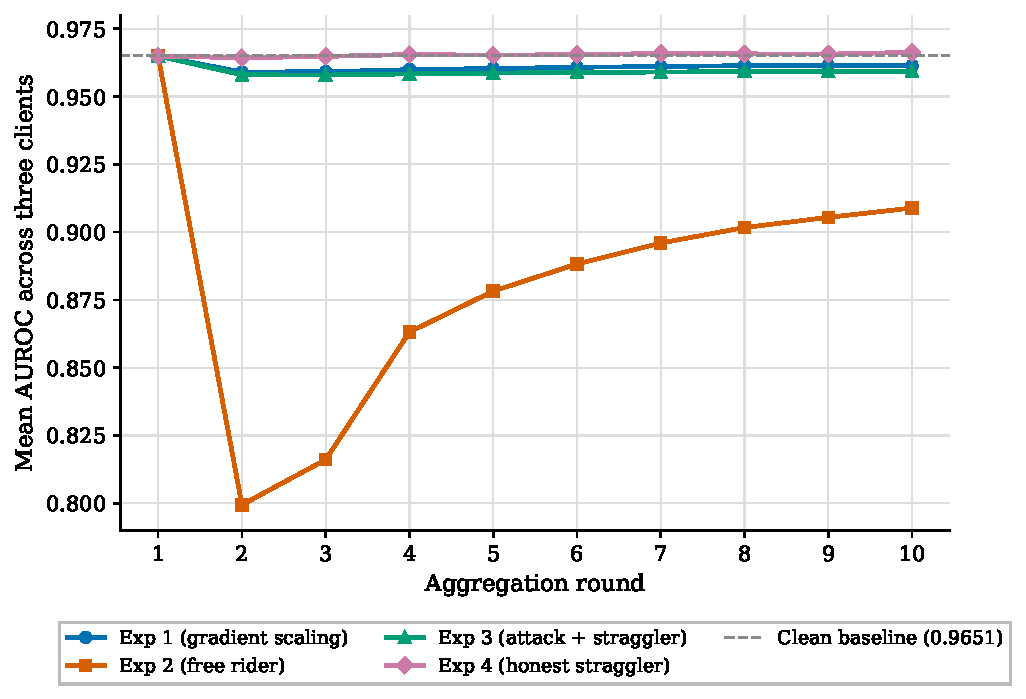
\includegraphics[width=\textwidth]{figures/fig_perround_auroc.pdf}
\caption{Per-round mean AUROC across the three client validation partitions (seed 42). The dashed line is the ten-seed clean baseline (0.9651), which is also the synchronous reference since every client submits within the window in that configuration. Exp~1/Exp~3 dip during warm-up and recover; Exp~2 shows the free-rider warm-up crash and subsequent recovery; Exp~4 tracks the baseline without false quarantine.}
\label{fig:perround}
\end{figure}

\subsection{Comparison against robust FL baselines}

Table~\ref{tab:baselines} compares SNAS against Krum, trimmed mean, and FLTrust. Krum obtains the highest raw AUROC in all three attack settings. However, server logs reveal that Krum selects Client 0 in \emph{every} aggregation round it performed: 300 of 300 selection decisions across Exp~1, Exp~2 and Exp~3 at ten seeds each, with zero exceptions. Beyond the raw win count, this outcome is itself a tie-break artifact rather than a genuine security property: at $N=3$, $f=1$, Krum's own validity condition $N\geq2f+3$ requires $N\geq5$, so this configuration sits outside its guarantee. With $k=\max(1,N-2)=1$, the two honest clients' scores are each the distance to the \emph{other} honest client — the same value for both, tied bit-for-bit — and Python's \texttt{min()} resolves the tie by insertion order, which favors whichever client submitted first (Client 0, at delay $0$s). Had submission order been adversarial, Krum would have selected the attacker instead. The Krum result is therefore not a federated aggregate; it is a repeated re-selection of one Medical ICU client, decided by submission order rather than by robustness. This can be beneficial for AUROC if that partition is sufficient for the task, but it discards the Surgical and Cardiac clients and defeats the purpose of collaborative federation.

Trimmed mean degenerates to vanilla FedAvg at $N=3$ with trim ratio 0.2 because $\lfloor 0.2\times3\rfloor=0$ coordinates are trimmed; it is therefore reported as a nominal rather than an effective robust baseline at this client count. The coordinate-wise median is the estimator that does not degenerate here: at $N=3$ it returns the middle value of every coordinate, so a single Byzantine client cannot move any coordinate past its honest neighbours regardless of perturbation size. We include it as the robust baseline trimmed mean was intended to be.

\paragraph{The median is a strong baseline, and beats SNAS under full participation.} This must be stated plainly rather than softened. On the two attacks in which all three clients submit within the window, the coordinate-wise median outperforms SNAS on both metrics and on every paired seed: $+0.0031$ AUROC on gradient scaling and $+0.0554$ on the free rider, each winning $10$ of $10$ seeds at the $n=10$ Wilcoxon floor ($p=0.00195$, paired $d=-13.3$ and $-8.1$). On the free rider it returns $0.9647$, statistically indistinguishable from the clean baseline --- the attack is neutralised outright. Any claim that SNAS dominates the robust-aggregation baselines at $N=3$ under full participation is not supported by these data.

\paragraph{But its guarantee is a function of who arrives.} The ordering reverses on Exp~3, the only setting in which a client straggles: there SNAS leads the median by $+0.0037$ AUROC, again $10$ of $10$ paired seeds ($p=0.00195$, $d=+6.7$), and the median is the weakest of all five aggregators. The mechanism is measurable rather than inferred. Client 2's $30$~s delay exceeds the $25$~s submission window, so it misses seven of ten rounds, and the server's own aggregation records show only two clients aggregated in those rounds. At $n=2$ the coordinate-wise median of two submissions \emph{is} their mean: the breakdown point $\lfloor (n-1)/2 \rfloor$ falls to zero and the $10\times$ attacker recovers its full $50\%$ influence. Across all thirty median runs, $90$ of $300$ rounds ($30.0\%$) aggregated only two clients and therefore carried no Byzantine tolerance at all.

This is the distinction the paper is actually about. Robust aggregation rules earn their guarantee from a quorum of honest submissions, so their breakdown point depends on how many clients \emph{arrive}; that is a synchronous-federation property. SNAS's staleness weighting and per-submission gating do not depend on the arrival count, and it is the only aggregator evaluated here that does not degrade when a client straggles. The claim we defend is therefore not that SNAS is the strongest robust aggregator, but that \textbf{quorum-dependent robustness degrades under asynchrony while per-submission detection does not}. It also yields a falsifiable prediction: at larger $N$ a single dropout no longer forces $n=2$, so the median's advantage should return and the Exp~3 gap should narrow.

FLTrust, by contrast, is a functioning baseline in this setting. The server computes a reference gradient by running its root split through the previous round's global encoder and the server head, then weights each client's \emph{update} $\Delta_i = \theta_i - \theta^g$ by $\mathrm{ReLU}(\cos(\Delta_i, g_{\mathrm{root}}))$. Two implementation details matter for reproducibility. First, the reference must be taken from the previous round's encoder, because the current global encoder is deliberately cleared while the submission window is open. Second, trust must be computed over updates rather than absolute weights: cosine similarity between full weight vectors is dominated by the shared base model, which leaves honest and adversarial submissions indistinguishable. With both handled, FLTrust produces three distinct, low-variance, attack-responsive results (Table~\ref{tab:baselines}) rather than collapsing onto the trimmed-mean values.

Figure~\ref{fig:baselines} visualizes these comparisons. The free-rider setting (Exp~2) is the one that separates the aggregators: SNAS exceeds FLTrust by $+0.033$ and trimmed mean by $+0.085$ AUROC, and the ordering of the standard deviations tracks the ordering of the means ($0.0070 < 0.0134 < 0.0189$), indicating that the methods which lose accuracy also become less stable across seeds. Krum's raw-AUROC lead, by contrast, coincides exactly with its collapse to single-client selection.

\begin{figure}[htbp]
\centering
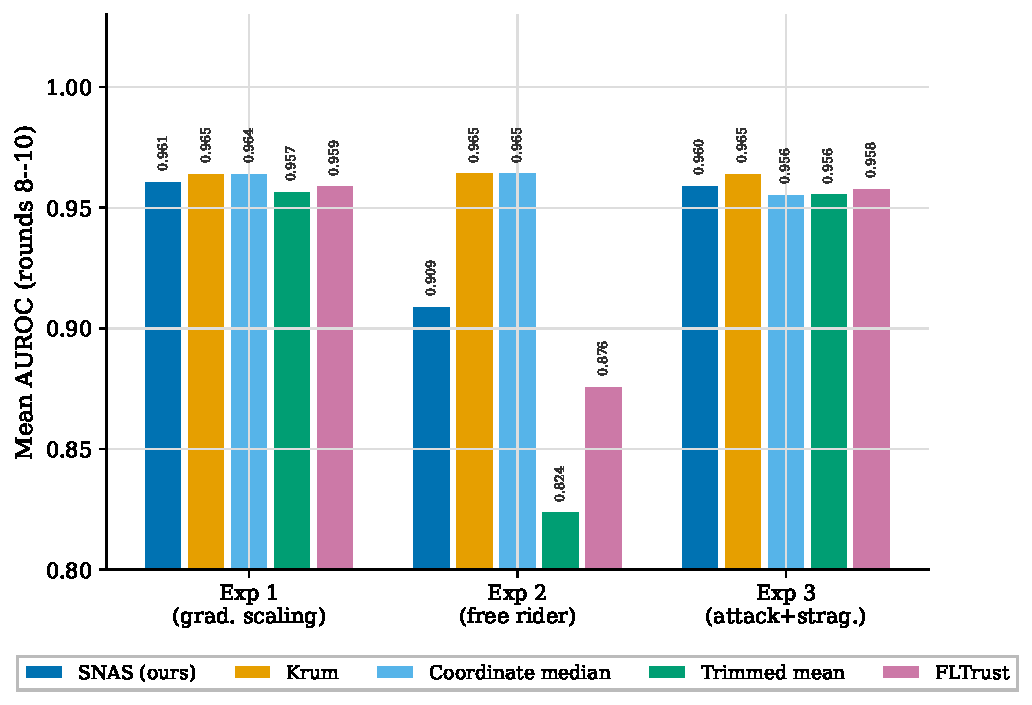
\includegraphics[width=0.9\textwidth]{figures/fig_baseline_comparison.pdf}
\caption{Aggregator comparison across Exp~1, Exp~2, and Exp~3. All bars are ten-seed means. Krum attains the highest raw AUROC but does so by selecting Client 0 in every aggregation round (300 of 300 selection decisions, zero exceptions) — a tie-break artifact of $N=3$ falling outside Krum's $N\geq2f+3$ validity condition, not a robustness property (Section~\ref{sec:n6}) — discarding the Surgical and Cardiac partitions. Exp~2 (free rider) is the setting that separates the aggregators: SNAS leads FLTrust by $+0.033$ and trimmed mean by $+0.085$ AUROC, each on ten of ten paired seeds.}
\label{fig:baselines}
\end{figure}

\begin{table}[htbp]
\caption{Baseline comparison. \textbf{All values are ten-seed means}, reported as AUROC~/~AUPRC per cell. Krum reaches higher raw AUROC but collapses federation by repeatedly selecting one client. The AUPRC column is the more discriminating one: on the free-rider attack (Exp~2) SNAS leads trimmed mean by $+0.085$ AUROC but by $+0.248$ AUPRC, and FLTrust by $+0.033$ AUROC but $+0.118$ AUPRC, so AUROC materially understates the separation between the aggregators at this prevalence.}
\label{tab:baselines}
\centering
\begin{tabularx}{\textwidth}{@{}lccc>{\raggedright\arraybackslash}X>{\raggedright\arraybackslash}X@{}}
\toprule
Aggregator & Exp~1 & Exp~2 & Exp~3 & Split-learning compatible? & Federation preserved? \\
 & \multicolumn{3}{c}{AUROC~/~AUPRC} & & \\
\midrule
SNAS & 0.9613~/~0.8357 & 0.9094~/~0.6723 & $\mathbf{0.9595}$~/~$\mathbf{0.8298}$ & Yes & Yes \\
Krum & 0.9646~/~0.8423 & 0.9647~/~0.8425 & 0.9646~/~0.8423 & Partially & No ($H=0$) \\
Coordinate median & $\mathbf{0.9644}$~/~$\mathbf{0.8457}$ & $\mathbf{0.9647}$~/~$\mathbf{0.8437}$ & 0.9559~/~0.8219 & Yes & Yes \\
Trimmed mean & 0.9569~/~0.8247 & 0.8242~/~0.4248 & 0.9560~/~0.8220 & Yes & Nominally \\
FLTrust & 0.9593~/~0.8290 & 0.8762~/~0.5548 & 0.9583~/~0.8261 & Yes & Nominally \\
\bottomrule
\end{tabularx}
\end{table}

All nine SNAS--baseline comparisons are statistically significant, and every one is decided unanimously across seeds. Against the two aggregators that genuinely federate, SNAS wins ten of ten paired seeds in all three experiments: over trimmed mean by $+0.0044$ (Exp~1), $+0.0852$ (Exp~2) and $+0.0035$ (Exp~3), and over FLTrust by $+0.0020$, $+0.0332$ and $+0.0013$ respectively. Against Krum the direction reverses, also ten of ten, by $-0.0033$, $-0.0553$ and $-0.0051$. Because every comparison is unanimous, each attains the two-sided Wilcoxon floor at $n=10$ ($p=0.00195$); the paired $t$-tests agree ($p$ from $3\times10^{-4}$ to $9\times10^{-10}$), with large paired effect sizes (Cohen's $d$ from $1.8$ to $8.2$ in magnitude). Effect sizes are computed as the mean paired difference divided by the standard deviation of those differences, the appropriate estimator for a paired design.

The Krum result should be read as a tradeoff between single-client selection and federation preservation, not as a universal superiority of Krum: as shown next, its entire advantage is obtained by discarding two of the three clients.

To make the federation-preservation argument quantitative rather than qualitative, we measure the \emph{contribution entropy} of each aggregator, defined per round as $H = -\sum_{i} \bar{\omega}_i \ln \bar{\omega}_i / \ln N$, where $\bar{\omega}_i$ is client $i$'s normalized aggregation share (as defined in Section~\ref{sec:agg}) and $N$ is the number of registered clients. $H=1$ indicates perfectly balanced participation and $H=0$ indicates that a single client carries the entire aggregate. Table~\ref{tab:entropy} reports the result, measured on the same runs that produce Table~\ref{tab:baselines} so that both aggregators are observed under identical conditions. Krum has $H=0.000$: all 300 of its selection decisions name Client 0 (the tie-break artifact discussed above, and confirmed as specific to $N=3$ in Section~\ref{sec:n6}), so its effective participation is a single client regardless of what the adversary does. SNAS has $H=0.986$ in the clean setting, matching to four decimal places the value predicted analytically from sample-count-proportional weighting, and falls to $H=0.767$, $0.685$ and $0.249$ on Exp~1, Exp~2 and Exp~3.

The direction of that reduction is the point. SNAS's entropy falls precisely because the gate withdraws weight from the client it has identified as adversarial --- the attacker's mean contribution share drops to $0.084$ on Exp~1 and $0.071$ on Exp~2 --- so the loss of balance is the defense operating as designed, and it varies with the attack. Krum's collapse is invariant: identical at $H=0.000$ across three different adversaries, because it is decided by submission order rather than by anything the adversary does. Exp~3 gives the lowest SNAS entropy ($0.249$) because two of the three clients are unavailable to the aggregate at once, one quarantined as malicious and one honestly straggling; this is a property of that experiment's design rather than of the aggregation rule.

\begin{table}[htbp]
\caption{Federation-preservation via contribution entropy $H\in[0,1]$ ($1$ = balanced participation, $0$ = single-client collapse). Mean normalized aggregation share per client, measured over 500 SNAS rounds (50 runs) and 300 Krum selection decisions (30 runs) from the same experiments as Table~\ref{tab:baselines}. SNAS's clean value reproduces the analytic sample-count-proportional prediction to four decimal places. Its entropy falls under attack because the gate withdraws weight from the detected adversary, and the reduction tracks which client is malicious; Krum's $H=0$ is instead identical across all three adversaries, being fixed by submission order. The no-detection ablation is the control: with the gate disabled its shares are the sample-count-proportional values under \emph{both} attacks, identical to the clean row, because it cannot withdraw weight from anyone. Attacker shares are shown in bold.}
\label{tab:entropy}
\centering
\begin{tabular}{lcccc}
\toprule
Setting & Client 0 & Client 1 & Client 2 & $H$ \\
 & share & share & share & \\
\midrule
SNAS, clean                & 0.39 & 0.25 & 0.35 & 0.986 \\
SNAS, Exp~1 (attacker C1)  & 0.48 & $\mathbf{0.08}$ & 0.44 & 0.767 \\
SNAS, Exp~2 (attacker C2)  & 0.56 & 0.37 & $\mathbf{0.07}$ & 0.685 \\
SNAS, Exp~3 (attacker C1, straggler C2) & 0.86 & $\mathbf{0.14}$ & 0.00 & 0.249 \\
\midrule
No-detection, Exp~1 and Exp~2 & 0.39 & 0.25 & 0.35 & 0.986 \\
Krum, Exp~1/2/3            & 1.00 & 0.00 & 0.00 & 0.000 \\
\bottomrule
\end{tabular}
\end{table}

\subsection{Validating the baselines at $N=6$}\label{sec:n6}

Two of the baselines above are evaluated outside their own validity conditions at $N=3$, and in both cases the cause is arithmetic rather than incidental. Krum selects the submission minimizing the sum of squared distances to its $k=N-f-2$ nearest neighbors; at $N=3$, $f=1$ this yields $k=0$, which the implementation clamps to $\max(1,N-2)=1$, and $N\geq2f+3$ is violated. Coordinate-wise trimmed mean discards $\lfloor \rho N \rfloor$ values per tail; at $\rho=0.2$ and $N=3$ this is $\lfloor 0.6 \rfloor = 0$, so the rule reduces exactly to the unweighted mean. At $N=6$ both conditions are satisfied without any change to the aggregation code: $k=3$ with no clamp, $N\geq2f+3$ holds, and the trimmed mean discards one value per tail. To establish that the $N=3$ Krum behavior reported above is an artifact of that regime rather than a property of the method, we repartition MIMIC-IV into six single-unit clients (MICU, MICU/SICU, SICU, TSICU, CCU, CVICU; $85{,}181$ stays retained) and rerun Exp~1 across all five aggregators at five seeds under an otherwise identical protocol.

Table~\ref{tab:n6-krum} reports the result that motivates the experiment. At $N=3$, Krum selects Client~0 in all $300$ of its selection decisions without exception; at $N=6$ it selects Client~0 in $1$ of $50$ decisions and distributes the remainder across three further honest clients. Critically, it never once selects the adversary. The $N=3$ behavior is therefore a tie-break artifact and not a selection criterion: with $k$ clamped to $1$, each honest client's score is its squared distance to the single other honest client, the two scores are bit-identical, and $\min$ resolves the tie by insertion order, which is fixed by submission order and hence by the configured delay. Client~0 submits at delay $0$\,s. Once $k=3$ the score is computed over a genuine neighborhood, the tie disappears, and Krum discriminates as designed. The accompanying change in accuracy confirms the reading: Krum \emph{falls} from $0.9646$ at $N=3$ to $0.9566$ at $N=6$ (Table~\ref{tab:n6-auroc}), so its apparent $N=3$ advantage over SNAS was produced by the artifact inflating it rather than by robustness. The same correction applies to trimmed mean, which is a genuine measurement here for the first time.

\begin{table}[htbp]
\caption{Krum selection distribution at $N=3$ and $N=6$ under Exp~1 (gradient scaling, adversary is Client~1 in both configurations). Counts are selection decisions: $300$ over ten seeds at $N=3$ and $50$ over five seeds at $N=6$. At $N=3$ Krum is outside its $N\geq2f+3$ condition and $k$ is clamped, making honest scores tie exactly so that the winner is fixed by submission order. At $N=6$ the clamp does not fire and selection spreads across four honest clients, never naming the adversary.}
\label{tab:n6-krum}
\centering
\begin{tabular}{lcc}
\toprule
Selected client & $N=3$ & $N=6$ \\
\midrule
Client 0                 & $\mathbf{300}$ (100\%) & 1 (2\%) \\
Client 1 (\emph{adversary}) & 0 & $\mathbf{0}$ \\
Client 2                 & 0 & 5 (10\%) \\
Client 3                 & --- & 18 (36\%) \\
Client 4                 & --- & 26 (52\%) \\
Client 5                 & --- & 0 \\
\midrule
Distinct clients selected & 1 & 4 \\
\bottomrule
\end{tabular}
\end{table}

\begin{table}[htbp]
\caption{Exp~1 (gradient scaling) at $N=6$, five seeds, compared against the ten-seed $N=3$ values from Table~\ref{tab:baselines}. The two federation sizes use different partitions and different client counts, so the columns are not paired and the comparison is between regimes rather than between matched runs. At $N=6$ all five aggregators fall within $0.003$ AUROC of one another. Trimmed mean and coordinate median agree to four decimals because with six submissions, trimming one per tail averages the middle four while the coordinate median is the midpoint of that same band; at $N=3$ they diverged only because the trimmed mean was degenerate.}
\label{tab:n6-auroc}
\centering
\begin{tabular}{lcc}
\toprule
Aggregator & $N=6$ (5 seeds) & $N=3$ (10 seeds) \\
\midrule
Trimmed mean      & $0.9580 \pm 0.0003$ & $0.9569 \pm 0.0005$ \\
Coordinate median & $0.9580 \pm 0.0004$ & $0.9644 \pm 0.0002$ \\
SNAS              & $0.9569 \pm 0.0002$ & $0.9613 \pm 0.0001$ \\
Krum              & $0.9566 \pm 0.0002$ & $0.9646 \pm 0.0005$ \\
FLTrust           & $0.9550 \pm 0.0002$ & $0.9593 \pm 0.0003$ \\
\bottomrule
\end{tabular}
\end{table}

On raw accuracy the five aggregators are separated by $0.003$ AUROC at $N=6$, with the two order statistics ahead of SNAS by roughly $0.001$; we therefore claim no accuracy advantage for SNAS in this configuration. We deliberately report no significance test here. This grid uses five seeds rather than the ten used throughout Section~\ref{sec:results}, and by the argument of Section~\ref{sec:setup} a five-seed paired Wilcoxon cannot reach conventional significance whatever the effect size, so a $p$-value would be uninformative rather than merely weak. The claim this section does make --- that Krum's single-client collapse is specific to $N=3$ --- rests on a count over $50$ selection decisions rather than on a comparison of means, and is unaffected by the seed budget. Gradient scaling is a magnitude attack that norm clipping, order statistics and reference-gradient weighting all address by construction, so it is the attack least able to separate correctly configured defenses --- consistent with Exp~1 being the narrowest margin in Table~\ref{tab:baselines} as well. The separation reported for SNAS arises on the free-rider attack (Exp~2), where it leads trimmed mean by $+0.085$ and FLTrust by $+0.033$ AUROC at $N=3$; that attack is not yet included in the $N=6$ grid, and extending the grid to it is the natural next step. What the $N=6$ grid does establish is narrower and was the reason for running it: the federation-collapse behavior attributed to Krum in Table~\ref{tab:entropy} is specific to the under-specified $N=3$ regime, and both Krum and trimmed mean are measured at their intended operating point here.

\subsection{Ablation: value of the anomaly gate}

The Byzantine-robust baselines above test the detection half of the design. To isolate what the anomaly gate itself contributes, we ablate it: disabling the SNAS gate and the norm-clipping step (setting both anomaly thresholds and the clip ratio to a value that never triggers) reduces the pipeline to a pure staleness-weighted asynchronous FedAvg with no anomaly detection. This ``no-detection'' condition is simultaneously the empirical asynchronous baseline a reader would expect --- staleness-weighted aggregation without a security mechanism --- and the ablation that quantifies the gate's benefit. We run it on all four experiments across the same ten seeds; Table~\ref{tab:ablation} reports the comparison, and Figure~\ref{fig:ablation} visualizes it.

\begin{table}[htbp]
\caption{Factorial ablation of the two defences, ten seeds per cell, all contrasts paired by seed. The four arms differ only in whether the anomaly gate and the norm clip are active; the configurations are otherwise identical, so seed $s$ shares its initialization and minibatch order across all four. ``Gate'' and ``clip'' are main effects, each averaged over the two levels of the other factor; ``inter.'' is the interaction $(\text{both}-\text{gate only})-(\text{clip only}-\text{neither})$, where a negative value means the two defences overlap. Every contrast on Exp~1--3 is unanimous over ten seeds at the $n=10$ Wilcoxon floor ($p=0.00195$), with paired Cohen's $d$ from $2.4$ to $14.5$.}
\label{tab:ablation}
\centering
\begin{tabular}{lcccccc}
\toprule
Experiment & Neither & Clip only & Gate only & Both & Gate & Clip \\
\midrule
Exp~1 gradient scaling & 0.9578 & 0.9596 & 0.9585 & $\mathbf{0.9613}$ & $+0.0012$ & $+0.0023$ \\
Exp~2 free rider & 0.8141 & 0.8585 & 0.9002 & $\mathbf{0.9094}$ & $+0.0685$ & $+0.0268$ \\
Exp~3 attack + straggler & 0.9567 & 0.9579 & 0.9570 & $\mathbf{0.9595}$ & $+0.0009$ & $+0.0019$ \\
Exp~4 honest straggler & 0.9658 & 0.9658 & 0.9658 & 0.9659 & $+0.0001$ & $+0.0000$ \\
\bottomrule
\end{tabular}
\end{table}

Four observations follow, three of which a two-corner ablation could not have produced.

First, the pipeline benefit is large and highly significant under the free-rider attack ($+0.0953$ AUROC from neither to both, ten of ten seeds), where unclipped random weights would otherwise corrupt the aggregate; the no-detection value ($0.8141$) sits close to the degenerate trimmed-mean result ($0.8242$), consistent with the pipeline reducing to vanilla FedAvg that absorbs the poison once detection is removed. Under gradient scaling and attack-plus-straggler the benefit is smaller ($+0.0035$ and $+0.0028$), because a uniformly scaled but directionally-honest update is partly diluted by staleness-weighted aggregation even without detection.

Second, \emph{which} defence carries that benefit depends on the attack, and the ordering reverses between them. Against the free rider the gate is worth roughly $2.5$ times the clip ($+0.0685$ against $+0.0268$); against gradient scaling and attack-plus-straggler the clip contributes more than the gate ($+0.0023$ against $+0.0012$, and $+0.0019$ against $+0.0009$). This is mechanically what one would expect --- a norm clip is precisely the right instrument against a $10\times$ scaled submission, while random weights are a direction anomaly no clip can repair --- but it is invisible unless the two factors are varied independently, and it means neither component is redundant.

Third, on the free rider the two defences are strongly \emph{sub-additive}: individually they are worth $+0.0861$ and $+0.0444$, but together only $+0.0953$, an interaction of $-0.0353$. They overlap, each recovering damage the other would also have caught. We report this rather than allow the two benefits to appear additive. On Exp~1 and Exp~3 the interaction is small and positive ($+0.0011$ and $+0.0013$), i.e.\ mildly complementary.

Fourth, neither defence costs anything when there is no attacker. On the honest-straggler experiment every contrast is at chance: win rates between four and six of ten seeds, $p$ between $0.23$ and $0.63$, and $|d|\leq0.45$. This is a proper null result, and it is the strongest available answer to the question of whether the gate induces false quarantines on benign stragglers. Together with the entropy result, it shows that SNAS is the only evaluated configuration that both keeps every honest client in the aggregate \emph{and} resists poisoning: Krum resists poisoning only by collapsing to a single client, while no-detection weights all clients but cannot exclude the attacker and so retains the poison.

\begin{figure}[htbp]
\centering
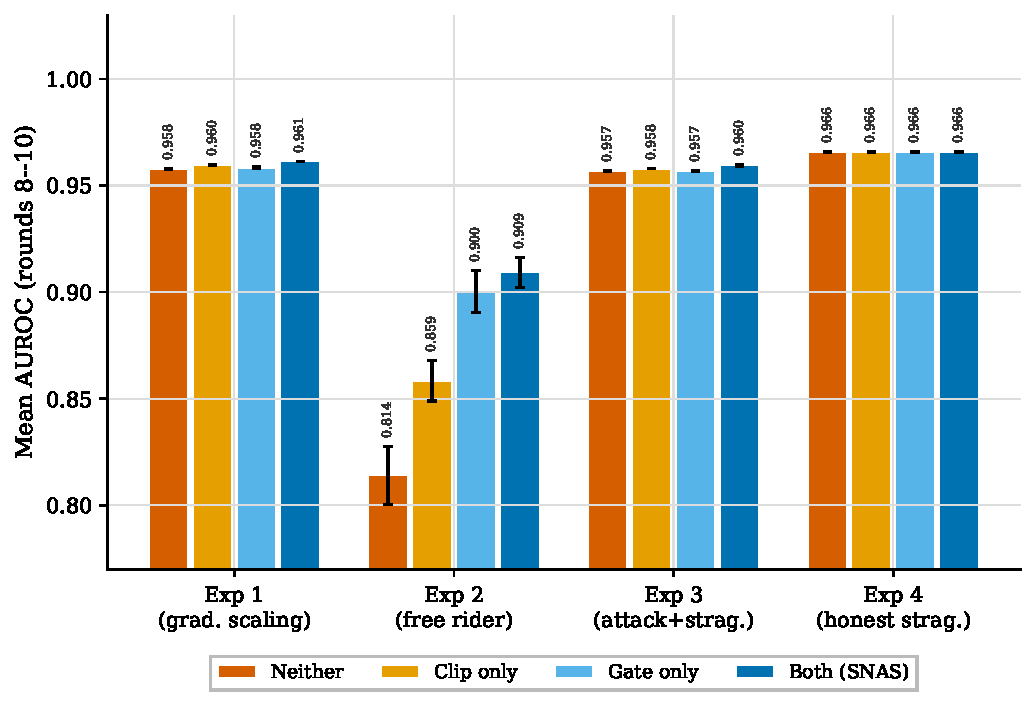
\includegraphics[width=0.75\textwidth]{figures/fig_ablation.pdf}
\caption{Gate ablation across the four experiments (ten-seed means, error bars are one standard deviation). Re-enabling the anomaly gate recovers substantial AUROC under the free-rider attack, a smaller but significant amount under gradient scaling and attack-plus-straggler, and nothing on the honest-straggler experiment (no attacker), demonstrating that the gate helps under attack without costing clean-case utility.}
\label{fig:ablation}
\end{figure}

\subsection{Adaptive adversary experiments}

Table~\ref{tab:adaptive} summarizes three adaptive attacks. A threshold-aware attacker that analytically targets 90\% of the quarantine threshold is still detected in every active detection round. The attack assumes no natural cosine drift, but ordinary local training drift pushes the true SNAS above the intended target.

A strategic alternation attacker, however, exposes a structural vulnerability. By attacking, then abstaining, then attacking again, the adversary ensures $\tau=1$ for each malicious submission. The $(1+\tau)$ denominator reduces the score enough to avoid the gate across all four staleness decay functions. This is a limitation of memoryless per-round scoring rather than a decay-function choice. The observed AUROC damage is modest in the evaluated setting, but the evasion itself is important.

The mechanism is visible in the scores rather than only in the outcome. The alternating attacker's mean SNAS is $0.175$--$0.177$ across the four decay functions, against a flag threshold of $0.22$: the halving induced by $\tau=1$ parks the score just below the gate, consistently and by a similar margin in every setting. The contrast with the threshold-aware attacker, whose mean score is $0.347$ and which is caught in every post-warm-up round, is what identifies the denominator rather than the decay function as the cause. The evasion is therefore systematic, not a marginal or noise-driven miss.

Slow-ramp mimicry is partially detected: the client is first flagged at round 10, detected in $38.5\%$ of post-warm-up rounds, never quarantined by round 15, and AUROC degradation remains small ($-0.0009$). This suggests that flagging and weight penalties can bound damage for gradual attacks, but hard quarantine may require temporal accumulation.

\begin{table}[htbp]
\caption{Adaptive adversary results, single seed. Detection is over post-warm-up attacker submissions; AUROC $\Delta$ is measured against the ten-seed clean asynchronous baseline of $0.9651$ (Table~\ref{tab:main-results}). ``Mean SNAS'' is the attacker's mean score over the same rounds, against $\delta_{\mathrm{flag}}=0.22$ and $\delta_{\mathrm{quarantine}}=0.35$; it shows directly why the alternating attacker evades, its score sitting just below the flag threshold in every decay setting. The alternation attack reveals a robustness boundary of memoryless staleness-normalized scoring.}
\label{tab:adaptive}
\centering
\begin{tabularx}{\textwidth}{@{}lcccc>{\raggedright\arraybackslash}X@{}}
\toprule
Attack & Detection & First detection & Mean SNAS & AUROC $\Delta$ & Interpretation \\
\midrule
Threshold-aware scaling & 100\% & Round 2 & 0.347 & $-0.0040$ & Formula-aware scaling fails due to training drift \\
Alternating, exponential & 0\% & Never & 0.177 & $-0.0038$ & Structural evasion \\
Alternating, linear & 0\% & Never & 0.175 & $-0.0037$ & Structural evasion \\
Alternating, polynomial & 0\% & Never & 0.175 & $-0.0037$ & Structural evasion \\
Alternating, step & 0\% & Never & 0.175 & $-0.0040$ & Worst damage among decay functions \\
Slow ramp, 15 rounds & 38.5\% & Round 10 & 0.221 & $-0.0009$ & Partial detection bounds damage \\
\bottomrule
\end{tabularx}
\end{table}

\subsection{Threshold calibration and held-out evaluation}\label{sec:calibration}

A detection threshold chosen by scanning for good detection and false-positive rates, and then evaluated by reporting those same rates, is calibrated on its own test set. To remove that circularity we fix $(\delta_{\mathrm{flag}}, \delta_{\mathrm{quarantine}})$ on a declared calibration set and evaluate on data that had no part in choosing them.

The calibration set is the clean runs together with the gradient-scaling attack (Exp~1) --- the setting the thresholds were originally tuned against --- across all ten seeds, giving 403 honest and 80 attacker client-rounds. Two mechanical rules are fixed in advance: $\delta_{\mathrm{flag}}$ is the highest honest SNAS observed in calibration plus a $5\%$ margin, the smallest threshold raising no false positive on calibration data; $\delta_{\mathrm{quarantine}}$ is the $25$th percentile of calibration attacker scores, rather than the minimum, which would fit the single lowest-scoring round. Applied to the calibration set these rules give $\delta_{\mathrm{flag}}=0.164$ and $\delta_{\mathrm{quarantine}}=0.346$.

Held out are the free-rider attack, the attack-plus-straggler setting, the label-flip attack and the backdoor attack, none of which contributed to the thresholds. On all four, detection is $100\%$ of post-warm-up attacker rounds, and the false-positive rate is $0\%$ on three of the four; the exception is the attack-plus-straggler setting, at $7.5\%$. Every attack is separable from honest behaviour by a margin of $0.09$--$0.28$ in SNAS. Repeating the exercise with a seed-disjoint split --- calibrating on five seeds and evaluating on the other five across all cells --- also gives $100\%$ detection at $0\%$ false positives, so the thresholds are not fitted to particular runs either.

Two conclusions follow, and the second is a limitation rather than a result. First, a \emph{single} flag threshold suffices for every attack studied: across all experiments the highest honest score is $0.195$ and the lowest attacker score is $0.233$, so any $\delta_{\mathrm{flag}}\in(0.195, 0.233)$ achieves $100\%$ detection at $0\%$ false positives on all of them simultaneously. The deployed value $0.22$ lies inside that window. It is also, notably, a better choice than the value the calibration rule produces: at $0.164$ the rule is too aggressive and induces the $7.5\%$ false-positive rate noted above, because honest scores in the straggler setting reach $0.195$. We therefore retain $0.22$ and report the derived value for transparency rather than adopting it. The window is only $0.038$ wide, which we state plainly: the choice is well founded but not generous, and a fifth attack family could narrow or close it.

Second, no single \emph{quarantine} threshold serves every attack. The derived $0.346$ independently reproduces the deployed $0.35$, so that value is not arbitrary --- but as Section~\ref{sec:results} reports, direction-driven attacks score $0.28$--$0.30$ while norm-driven attacks score $0.36$--$0.42$, and $\delta_{\mathrm{quarantine}}$ falls between them. The consequence is that label-flip and backdoor submissions are flagged in every round yet quarantined in almost none. This is a property of the score, not of the calibration: recalibrating cannot separate two attack families whose score distributions do not separate. A per-signal threshold, or a score normalised so that direction and magnitude anomalies are commensurable, is the appropriate remedy and we identify it as future work.

\subsection{Hyperparameter sensitivity}

Table~\ref{tab:sensitivity} summarizes the sensitivity analysis, over 139 single-seed grid points. Detection on the gradient-scaling setting is stable for $\beta\in[0.10,0.70]$ when $\gamma=1-\beta$, corresponding to 77.8\% of the tested range. Detection degrades only when $\beta\geq0.80$, where the norm-anomaly component is too heavily downweighted --- falling to 71.4\% at $\beta=0.80$ and 42.9\% at $\beta=0.90$. Threshold sweeps over 115 valid $(\delta_{\mathrm{flag}},\delta_{\mathrm{quarantine}})$ combinations show that 71 combinations, or 61.7\%, achieve 100\% detection with 0\% false positives on the hardest evaluated Exp~3 setting. Clip ratio sensitivity from 1.5 to 4.0 shows identical 100\% DR and 0\% FPR across all tested values.

The $\beta$ constraint is imposed by one attack family and not the other, which is what makes the safe range interpretable rather than merely empirical. Sweeping $\beta$ on the free-rider attack gives $100\%$ detection at \emph{every} tested value, $0.10$ through $0.90$, with no false positives; sweeping it on gradient scaling gives $100\%$ only up to $0.70$. The asymmetry follows from the attacks' signatures. A free rider submits random weights, which are anomalous in direction and magnitude simultaneously, so either term alone suffices and the split between them is immaterial. Gradient scaling is a pure magnitude attack that the cosine term cannot see at all, so it depends entirely on $\gamma=1-\beta$ remaining large enough; once $\beta\geq0.80$ the norm term is too heavily downweighted and detection falls, reaching $42.9\%$ at $\beta=0.90$, where the sweep also records its only false positives ($7.7\%$). The upper bound of the safe range is therefore set by the norm-driven attack, and $\beta=0.35$ sits comfortably inside the region where both families are detected.

This sweep was regenerated on the 265-feature data after the removal of \texttt{los}, so it rests on the same feature set as every other result reported here. The regeneration left all three conclusions unchanged: the same $\beta$ safe range, the same 71 of 115 threshold pairs, and the same insensitivity to the clip ratio, with absolute AUROC shifting by less than $0.002$ throughout. The one difference is that detection past $\beta=0.70$ degrades slightly more sharply on the corrected data than on the earlier feature set, which strengthens rather than weakens the case for the chosen operating point. Figure~\ref{fig:heatmap} shows the threshold sweep as two panels: detection rate (uniformly $100\%$ across the valid region) and false-positive rate (the quantity that actually varies). The zero-FPR region is a broad plateau rather than a knife-edge, and the default operating point sits comfortably inside it.

\begin{figure}[htbp]
\centering
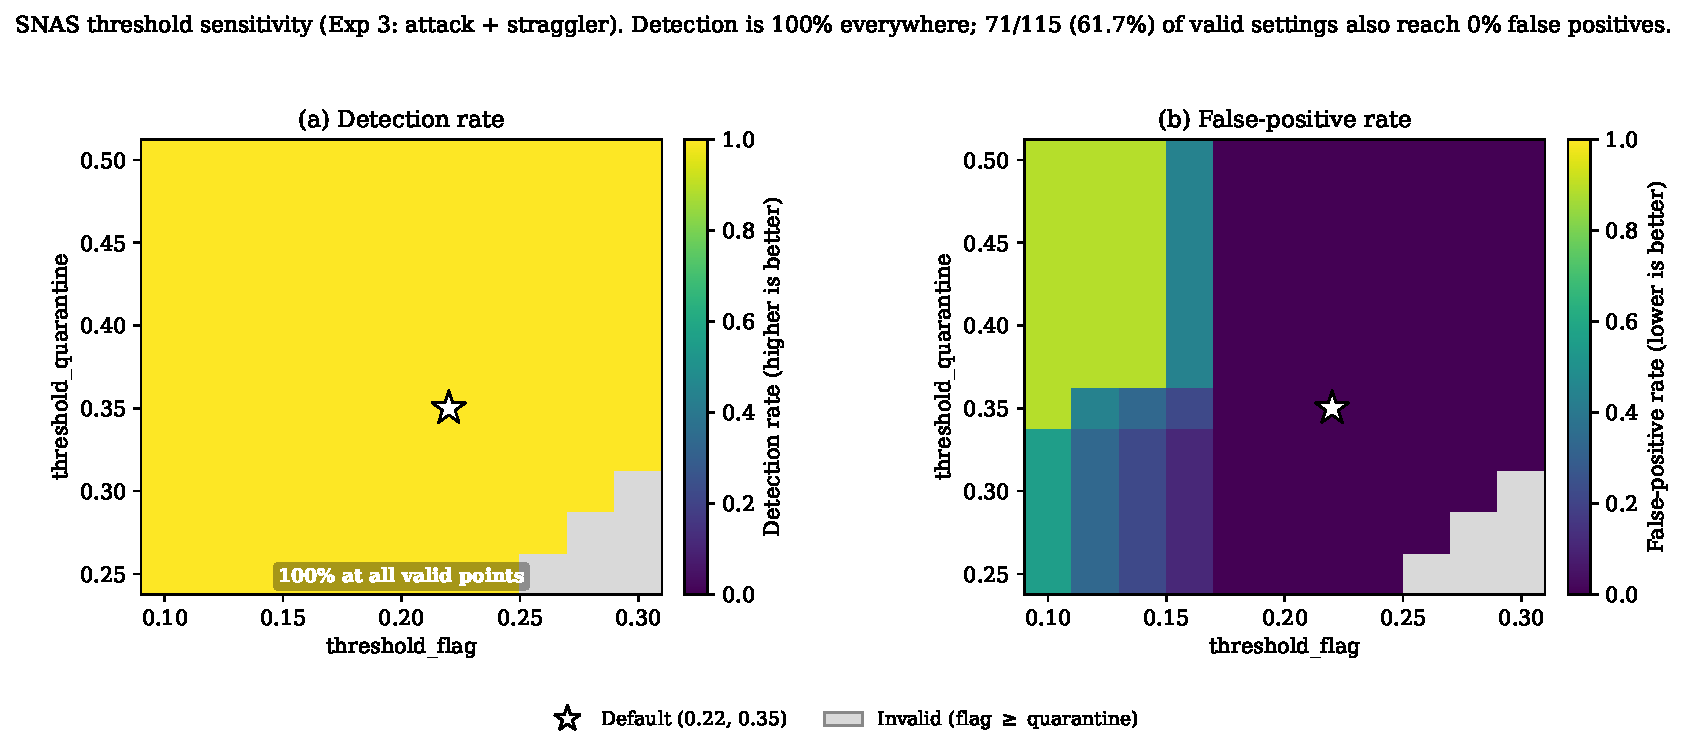
\includegraphics[width=\textwidth]{figures/fig_sensitivity.pdf}
\caption{Threshold sensitivity on the Exp~3 (attack + straggler) setting, over the $(\delta_{\mathrm{flag}},\delta_{\mathrm{quarantine}})$ grid. \textbf{(a)} Attacker detection rate is uniformly $100\%$ at every valid setting, so this panel is intentionally uniform. \textbf{(b)} The false-positive rate is the quantity that varies: the large dark region marks the zero-FPR operating zone, which covers $71/115$ ($61.7\%$) of valid settings. The star marks the reported default $(0.22,0.35)$, which lies well inside the zero-FPR zone. Grey cells are invalid combinations where $\delta_{\mathrm{flag}}\geq\delta_{\mathrm{quarantine}}$ (not evaluated), and are distinct from a value of zero. The broad zero-FPR plateau shows the operating point is not a knife-edge.}
\label{fig:heatmap}
\end{figure}

\begin{table}[htbp]
\caption{Hyperparameter sensitivity summary, 139 single-seed grid points on the 265-feature data. The $\beta$ and clip-ratio rows are measured on the Exp~1 gradient-scaling setting and the threshold row on the harder Exp~3 attack-plus-straggler setting.}
\label{tab:sensitivity}
\centering
\begin{tabular}{lll}
\toprule
Parameter & Safe operating range & Summary statistic \\
\midrule
$\beta$ (gradient scaling) & 0.10--0.70 & 77.8\% of tested values retain 100\% DR \\
$\beta$ (free rider) & 0.10--0.90 & All tested values retain 100\% DR \\
Threshold pair & 71/115 valid pairs & 61.7\% retain 100\% DR and 0\% FPR \\
Clip ratio & 1.5--4.0 & All tested values retain 100\% DR and 0\% FPR \\
\bottomrule
\end{tabular}
\end{table}

\subsection{Attack-magnitude sensitivity}\label{sec:attack-magnitude}

The detection rates reported above are all measured at a single, strong attack magnitude ($10\times$ gradient scaling, or fully random free-rider weights). Two questions follow. First, whether the observed $100\%$ detection reflects a genuinely discriminative gate or merely the choice of an extreme attack. Second, whether an adversary can evade the gate by scaling the encoder \emph{down} rather than up. The second question matters because the norm term in Equation~(9) is defined on $\left|\log(\|\theta_{i,k}\|/\|\theta^g_k\|)\right|$, and is therefore symmetric about a scale of $1.0$ by construction: a $0.1\times$ downscale and a $10\times$ upscale should produce the same norm anomaly. We test both by sweeping the gradient-scaling factor on the Exp~1 setup from $0.1\times$ to $10\times$, spanning an order of magnitude in each direction, with all detector parameters at their defaults. Table~\ref{tab:attack-magnitude} reports the resulting detection curve.

\begin{table}[htbp]
\caption{Attack-magnitude sweep on the Exp~1 gradient-scaling setup (single seed, all detector parameters at defaults), spanning an order of magnitude of both downscaling and upscaling. Detection rate is over the attacker's eight post-warm-up rounds. Detection is high at both ends of the range and falls to zero only in a band around $1.0\times$, where the submitted encoder is close to honest; within that band the attack also causes negligible degradation.}
\label{tab:attack-magnitude}
\centering
\begin{tabular}{lllll}
\toprule
Scale & AUROC (R8--10) & Round-1 AUROC drop & Detection rate & First detection \\
\midrule
$0.1\times$ & 0.9642 & 0.0021 & 100\% & Round 2 \\
$0.3\times$ & 0.9638 & 0.0021 & 12.5\% & Round 3 \\
$0.5\times$ & 0.9651 & 0.0019 & 0\% & -- \\
$0.8\times$ & 0.9655 & 0.0021 & 0\% & -- \\
$1.2\times$ & 0.9651 & 0.0022 & 0\% & -- \\
$1.5\times$ & 0.9643 & 0.0025 & 0\% & -- \\
$2.0\times$ & 0.9631 & 0.0028 & 0\% & -- \\
$3.0\times$ & 0.9628 & 0.0032 & 37.5\% & Round 3 \\
$5.0\times$ & 0.9621 & 0.0042 & 100\% & Round 2 \\
$7.0\times$ & 0.9613 & 0.0050 & 100\% & Round 2 \\
$10.0\times$ & 0.9614 & 0.0059 & 100\% & Round 2 \\
\bottomrule
\end{tabular}
\end{table}

The detection curve is U-shaped in the scale factor, and is visualized in Figure~\ref{fig:attack-magnitude}. Detection is $100\%$ at $0.1\times$ and at $5\times$ and above, falls to zero across the band from $0.5\times$ to $2.0\times$, and passes through partial-detection transitions at $0.3\times$ ($12.5\%$) and $3\times$ ($37.5\%$). This is the behaviour Equation~(9) predicts: what the gate responds to is the magnitude of the log-ratio between the submitted and global norms, not its sign, so shrinking the encoder is detected on the same terms as inflating it. The symmetry is close but not exact --- $0.5\times$ and $2.0\times$ both evade, and $0.1\times$ and $10\times$ are both fully detected, whereas $0.3\times$ is detected less often than $3\times$ despite a marginally larger log-deviation --- because the cosine term also contributes to SNAS and responds differently to the two directions.

Two consequences follow. First, the downscaling attack is not an evasion route: an adversary that shrinks the encoder by an order of magnitude is flagged in every post-warm-up round, and the score is symmetric by construction rather than by tuning. Second, the residual evasion band is narrow and benign. Within $0.5\times$--$2.0\times$ the round-1 AUROC drop stays between $0.0019$ and $0.0028$, no larger than the $0.0021$ observed at the fully-detected $0.1\times$ point and comparable to ordinary run-to-run variation; the mean AUROC over rounds 8--10 varies by under $0.003$ across the entire swept range. The attacks SNAS does not flag are therefore those that barely perturb the aggregate, while every attack large enough to move it is caught. This indicates that the $100\%$ detection reported elsewhere reflects the gate's discrimination rather than the choice of a single extreme magnitude.

One asymmetry is worth stating precisely, because it bounds the claim. Hard quarantine is triggered only at $10\times$; at $0.1\times$, $5\times$ and $7\times$ the attacker is flagged in every active round and has its aggregation weight penalised, but never crosses the quarantine threshold $\delta_{\mathrm{quarantine}}=0.35$. Detection and exclusion are therefore not the same event, and the $100\%$ figures in this table refer to detection.

\begin{figure}[htbp]
\centering
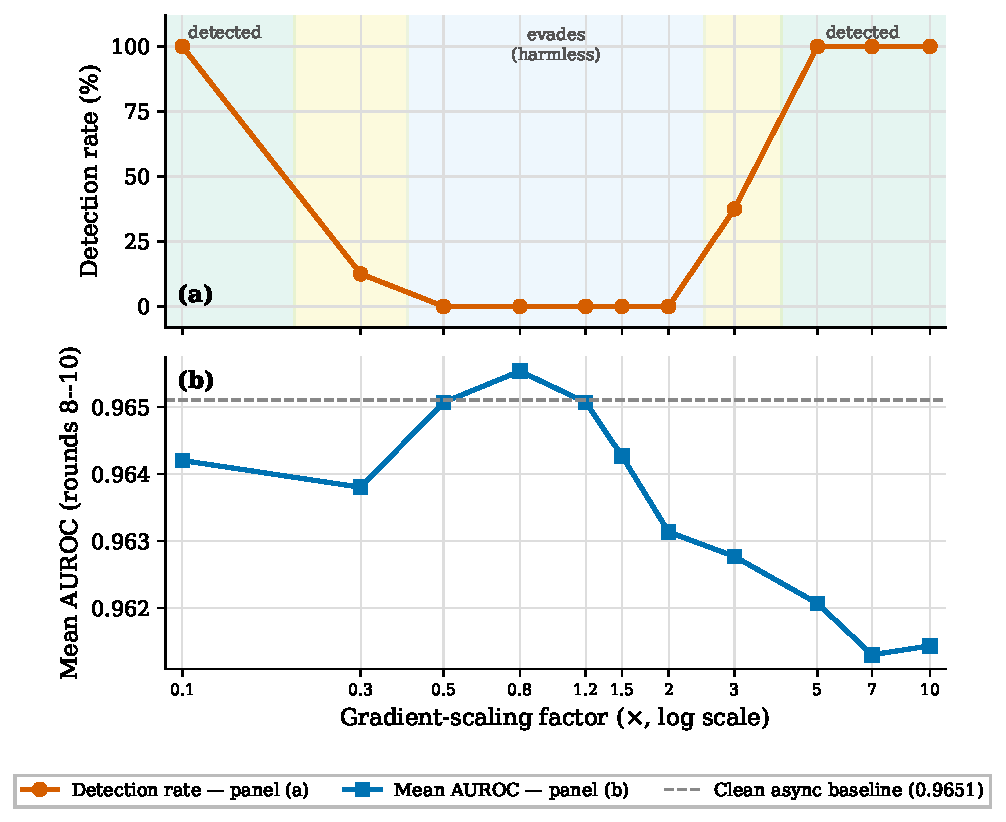
\includegraphics[width=0.72\textwidth]{figures/fig_attack_magnitude.pdf}
\caption{Attack-magnitude sweep on Exp~1, spanning $0.1\times$ to $10\times$ on a logarithmic scale axis. (a) Attacker detection rate is U-shaped: $100\%$ at both ends, zero across the $0.5\times$--$2.0\times$ band, with partial-detection transitions at $0.3\times$ and $3\times$. Downscaling is detected on the same terms as upscaling, as the symmetric norm term in Equation~(9) predicts. (b) Mean AUROC varies by under $0.003$ across the full range. The attacks that evade detection are those that barely move AUROC, so the evasion band coincides with the absence of meaningful harm.}
\label{fig:attack-magnitude}
\end{figure}

\subsection{Communication cost}

SENTINEL-SplitFed adds no additional client-server communication beyond the underlying SplitFed protocol. Per batch, each client sends a $64\times32$ activation tensor and receives a gradient tensor of the same size, corresponding to 8,192 bytes each with 32-bit floats. With 200 batches per round, this gives 3,276,800 bytes per client per round and 9,830,400 bytes for three clients per round. Over 10 rounds, activation-gradient exchange totals 98,304,000 bytes. Encoder transfer for aggregation remains approximately 77 KB per client per round. SNAS computation, staleness tracking, gating, and aggregation all occur server-side.

\section{Discussion}\label{sec:discussion}

\subsection{Why raw AUROC is not sufficient}

The Krum comparison is the most important interpretive result. If the only metric is AUROC, Krum appears superior. However, its behavior is closer to client selection than federated aggregation in this low-client non-IID setting. Repeatedly selecting Client 0 can perform well when that partition is predictive, but it eliminates contributions from Surgical and Cardiac clients. This is made explicit by the contribution-entropy metric (Table~\ref{tab:entropy}): Krum operates at $H=0.000$ in every round of every experiment (single-client collapse), while SNAS operates at $H=0.986$ when no attacker is present and reduces entropy only in proportion to how much weight it withdraws from a detected adversary. The gate ablation (Table~\ref{tab:ablation}) completes the picture: the no-detection baseline weights all clients but cannot exclude the attacker, so it retains the poison and loses accuracy under the free-rider attack. SNAS is thus the only evaluated configuration that simultaneously keeps every honest client in the aggregate and resists poisoning. For critical-care federation this matters because the objective is not merely to maximize a global validation number, but to learn collaboratively across heterogeneous clinical domains. Further per-domain AUROC and minimum-contribution-rate reporting are natural complements for future multi-institution deployments.

\subsection{Why the detector scores absolute weights rather than updates}\label{sec:basis}

A natural objection to the cosine term of the Staleness-Normalized Anomaly Score (Section~\ref{sec:method}) is that $\cos(\theta_i, \theta^g)$ is dominated by the shared base model: every client begins the round \emph{from} $\theta^g$ and takes a small step, so $\theta_i = \theta^g + \Delta_i$ with $\lVert\Delta_i\rVert \ll \lVert\theta^g\rVert$, and the cosine is close to unity for honest and adversarial clients alike. The objection is correct about the mechanism. It does not, however, follow that scoring the update $\Delta_i$ instead would detect better, and at this federation size it detects appreciably worse.

We tested this directly. A parallel arm recomputes both weight signals on $\Delta_i$, referenced against the mean \emph{direction} of the other clients' updates, leaving everything else identical --- same seeds, same attacks, gate disabled in both arms so that at each seed the two bases are scored on the same training trajectory (their final AUROCs agree to four decimal places). Because the gate never fires, this compares the separability of the score itself rather than a threshold calibrated for one basis and applied to the other. We therefore report the rank-based AUC of the score and the detection rate attainable at zero false positives, which is what a perfectly recalibrated threshold could achieve.

The absolute basis separates attacker from honest observations perfectly on all three attacks (AUC $1.000$, $100\%$ detection at zero false positives). The update basis matches it only on the free rider; on gradient scaling it falls to $12.5\%$ detection at zero false positives (AUC $0.891$), and on the attack-plus-straggler setting it is \emph{at chance} (AUC $0.514$). Two mechanisms account for this, and both are properties of the client count rather than of the implementation.

First, the peer reference is itself attackable at $N=3$. Each honest client's leave-one-out reference comprises one honest peer and the attacker, so the adversary contributes half of the reference against which everyone else is judged. This lifts honest scores far more than the attacker's --- from $0.161$ to $0.306$ on gradient scaling --- collapsing the separation ratio from $2.30$ to $1.37$. An earlier variant using the raw peer mean was worse still: a $10\times$ attacker produces an update roughly $900$ times the honest norm, so the two-peer mean is essentially the attacker's own vector and the honest clients score \emph{above} it, inverting the ranking entirely.

Second, and decisively, at $n=2$ the update-space signal carries no information at all, and provably so. With a single peer $j$, the reference for client $i$ is $\Delta_j/\lVert\Delta_j\rVert$, so
\[
A^{\mathrm{cos}}_i = 1 - \cos(\Delta_i, \Delta_j) = A^{\mathrm{cos}}_j
\]
by symmetry of the cosine, and the norm term degenerates identically since $\lvert\log(a/b)\rvert = \lvert\log(b/a)\rvert$. Attacker and honest client receive \emph{identical} scores. This is confirmed in the logs: in every round of the straggler experiment where one client misses the window, the two remaining clients record byte-identical cosine and norm anomalies. Since $30\%$ of rounds in that setting aggregate only two clients, the chance-level AUC is the expected outcome rather than an anomaly.

One exclusion in this arm should be stated explicitly. Because the gate is disabled throughout the parallel arm, so that the two bases are compared on identical training trajectories, the $10\times$ attacker compounds unchecked and the encoder exceeds the range of single-precision floating point by the eighth round; $40$ update-basis scores in the straggler experiment ($4$ per seed, all in that setting) are consequently not finite and are excluded from the AUC computation rather than imputed. The absolute basis never encounters this, because the cap $\min(\lvert\log(\cdot)\rvert/\log 100, 1)$ absorbs an unbounded norm ratio by construction. The excluded observations fall in rounds where only two clients submitted, which the symmetry argument above already shows carry no signal in update space, so they cannot alter the conclusion; we report the count rather than silently dropping them.

The absolute basis is immune to both failures because its reference --- the previous round's global encoder --- is an anchor that the current round's attacker cannot influence and that exists regardless of how many clients arrived. This is the detection-side counterpart of the aggregation-side result in Section~\ref{sec:results}: peer-referenced robustness and peer-referenced detection both lose their guarantee when the peer set shrinks under asynchrony, while anchored alternatives do not. We therefore retain the absolute basis, and note that both effects should weaken as $N$ grows, since the reference stops being half adversary and a single dropout no longer forces $n=2$.

\subsection{Robustness boundary of memoryless SNAS}

The strategic alternation attack shows that staleness normalization must be designed carefully. The same denominator that protects honest stragglers can be exploited by a client that deliberately misses rounds before submitting poisoned updates. This does not invalidate SNAS, but it clarifies the threat model: memoryless per-round gates are insufficient against adversaries that manipulate their own participation schedule.

However, this vulnerability is inherently self-limiting, because the staleness counter $\tau$ enters the framework in two places with opposing effects for the attacker. In the detection gate, $\tau$ appears in the denominator $1/(1+\tau)$, so increasing $\tau$ lowers the SNAS score and aids evasion. But $\tau$ \emph{also} governs the aggregation weight through the staleness decay $d(\tau)$ (Section~\ref{sec:agg}): a stale submission is weighted by $d(\tau)$, which \emph{decreases} in $\tau$. An attacker therefore cannot raise $\tau$ to shrink its detection score without simultaneously shrinking its influence on the aggregate. Moreover, to hold a fixed staleness $\tau$ at every malicious submission, the adversary must abstain for $\tau$ rounds between attacks, so it poisons at most a $1/(1+\tau)$ fraction of rounds. The effective poisoning power --- the product of attack frequency and per-submission aggregation weight --- therefore collapses as $\tau$ grows.

\begin{table}[htbp]
\caption{Evasion--influence tradeoff for the attack-then-abstain adversary under the default exponential decay $d(\tau)=e^{-0.5\tau}$. A larger $\tau$ lowers the SNAS score (aiding evasion) but simultaneously lowers both the attack frequency and the per-submission aggregation weight, so the effective poisoning power collapses.}
\label{tab:tradeoff}
\centering
\begin{tabular}{ccccc}
\toprule
Staleness $\tau$ & SNAS factor $\tfrac{1}{1+\tau}$ & Attack frequency & Agg.\ weight $d(\tau)$ & Effective poisoning $\propto$ freq $\times\, d(\tau)$ \\
\midrule
1 & 0.50 & 1/2 & 0.61 & 0.30 \\
2 & 0.33 & 1/3 & 0.37 & 0.12 \\
3 & 0.25 & 1/4 & 0.22 & 0.056 \\
6 & 0.14 & 1/7 & 0.05 & 0.007 \\
7 & 0.13 & 1/8 & 0.03 & 0.004 \\
\bottomrule
\end{tabular}
\end{table}

Table~\ref{tab:tradeoff} makes this explicit under the default exponential decay. The attack-then-abstain strategy is most damaging at $\tau=1$ --- the minimum abstention that still yields the evasion benefit --- which is exactly the configuration evaluated in Table~\ref{tab:adaptive}, where the AUROC degradation is only $-0.004$. Pushing $\tau$ to $6$ or $7$ shrinks the SNAS score further, but the attacker then submits only once every seven or eight rounds, and each submission carries roughly $3$--$5\%$ weight, reducing effective poisoning power by more than an order of magnitude relative to $\tau=1$. Under step decay the attacker retains full weight while $\tau$ stays within the cutoff (which is why step decay shows the largest damage in Table~\ref{tab:adaptive}), but any $\tau$ beyond the cutoff removes it from aggregation entirely. The staleness-normalized gate thus admits an evasion window, yet the same staleness that opens it caps the harm an evading attacker can inflict.

A natural mitigation is temporal accumulation. For example, the server can maintain an exponential moving average
\begin{equation}
    M_i(r) = \lambda M_i(r-1) + (1-\lambda)\mathrm{SNAS}_i(r),
\end{equation}
or separately accumulate the numerator terms before staleness normalization. Another mitigation is to apply staleness dampening only to activation- or drift-related components, while leaving norm-anomaly evidence less dampened. A third option is to cap the denominator, e.g., $1+\min(\tau_i,\tau_{\max})$, so repeated short absences cannot fully neutralize anomaly evidence.

\subsection{Scope and limitations}\label{sec:limitations}

This study has eight main limitations. First, the primary benchmark uses three clients, reflecting a realistic low-client healthcare federation but limiting conclusions about large-scale cross-device FL. This bound is also what places Krum outside its own $N\geq2f+3$ validity condition and reduces the trimmed mean to an unweighted average, so the $N=3$ comparison characterizes both baselines in an under-specified regime rather than at their intended operating point. Section~\ref{sec:n6} addresses this for the gradient-scaling attack by repartitioning into six clients, where both conditions are satisfied and Krum's single-client collapse does not reproduce; the remaining attack settings, including the free-rider attack on which SNAS's separation is largest, are evaluated at $N=3$ only. Sweeps over the fraction of malicious clients, which require $N\geq5$ to be meaningful at $f\geq2$, are likewise not attempted here.

Second, and most important for interpreting the absolute predictive numbers, \textbf{the benchmark is not a clinically valid mortality model and its AUROC should not be compared against the published MIMIC-IV literature}. As detailed in Section~\ref{sec:setup}, features are aggregated over the whole admission and whole ICU stay with no early observation window, so for non-survivors the feature window extends through terminal deterioration; and the train/validation split is at row level rather than patient or admission level, so ICU stays belonging to the same admission can appear on both sides carrying identical laboratory blocks and identical labels. Both effects inflate AUROC. Excluding length of stay removes the single most direct leak but does not remove these two. A clinically comparable benchmark would require a fixed early observation window (for example, first-24-hour features) and a group-aware split on \texttt{subject\_id}, together with a held-out test set; we did not run that variant here. Because every aggregator is evaluated on the identical pipeline, the \emph{relative} security findings that constitute this paper's contribution are unaffected, but the absolute number is a property of the substrate rather than a clinical result.

Third, the sensitivity sweep is single-seed for compute tractability, although the main attack settings are repeated over ten seeds. Fourth, SNAS evaluates encoder submissions but does not provide cryptographic privacy or formal Byzantine guarantees. Fifth, the threat model covers encoder-submission attacks only: poisoning of the server-side top model $g_\phi$ during split training is out of scope and undefended, as stated in Section~\ref{sec:problem}. Sixth, the current adaptive mitigation is discussed but not fully implemented as a new defense.

Seventh, and important for how the federated setting itself should be read: \textbf{this is a single-centre benchmark, and its clients are not independent institutions}. MIMIC-IV is collected at one hospital, so the partitions used here are care units within a single centre --- sharing one electronic health record system, one laboratory, one set of clinical protocols and one patient catchment. Partitioning by ICU unit yields genuine covariate and prevalence heterogeneity, and mortality prevalence spans a factor of $2.3$ across the three clients, which is the non-IID stress the aggregation methods are evaluated against. But it is a \emph{proxy} for cross-institutional heterogeneity, not an instance of it: real hospitals differ additionally in coding practice, instrumentation, case mix and data quality, and those differences are exactly the ones that make federated learning necessary rather than merely convenient. We therefore claim only that SNAS is evaluated under realistic within-centre non-IID conditions, and not that it has been validated across institutions. Multi-centre validation on a second, genuinely multi-hospital corpus such as eICU is the natural next step and is left to future work.

Eighth, the attack suite is not exhaustive. We evaluate six settings spanning magnitude-based (gradient scaling), direction-based (free rider, label-flip proxy, backdoor) and adaptive SNAS-aware adversaries (threshold-aware, strategic alternation, slow ramp), which is broader than the two attack types the design was originally tuned against. It nonetheless omits the standard optimisation-based Byzantine attacks from the federated-learning literature --- in particular ALIE-style perturbations calibrated to the honest submissions' empirical variance, and Fang-style attacks optimised against a known aggregation rule. Both are most damaging when the honest population is large enough for an adversary to hide inside its variance, so a three-client federation is the regime least suited to evaluating them fairly; adding them alongside the $N=6$ configuration of Section~\ref{sec:n6} is the natural extension.

Additionally, staleness is measured as missed participation rather than model-version divergence, as detailed in Section~\ref{sec:method}; a version-based formulation would strengthen the asynchronous claims and is left to future work.

These limitations point directly to future work on windowed and group-split benchmark construction, multi-centre validation, distributed deployment with genuine timing measurement, version-based staleness, larger client counts, standard optimisation-based attack suites, server-head defenses, temporal anomaly memory, and privacy-enhancing split-learning mechanisms.

\section{Conclusion}\label{sec:conclusion}

We introduced SENTINEL-SplitFed, a server-side framework for asynchronous split federated learning with intrusion resilience in critical-care mortality prediction. The method combines timed aggregation windows, staleness tracking, staleness-normalized anomaly scoring, norm clipping, and gate-based robust aggregation. On non-IID MIMIC-IV clients, SENTINEL-SplitFed preserves clean asynchronous performance, avoids false quarantine of honest stragglers, and detects evaluated gradient-scaling and free-rider attacks with 100\% detection of post-warm-up attacker submissions (8/8; 80\% including the warm-up rounds) and 0\% observed false positives (0/16 honest client-rounds). Baseline comparisons reveal that standard robust FL methods require care before they transfer to low-client SplitFed. In the three-client regime Krum collapses federation to a single client and the trimmed mean degenerates to an unweighted average; both are consequences of that regime rather than of the methods, and both resolve once the federation is repartitioned into six clients, where Krum discriminates genuinely and never selects the adversary. FLTrust is compatible with split-learning encoder aggregation, but only once its reference gradient is derived from the previous round's global encoder and trust is computed over updates rather than absolute weights; without both adaptations it silently degenerates to uniform averaging. Adaptive attacks also reveal a clear robustness boundary, motivating temporal SNAS accumulation. Overall, SENTINEL-SplitFed provides a practical and empirically grounded step toward resilient split federated learning for critical healthcare applications.

\backmatter

\section*{Declarations}

\bmhead{Funding} This work was not supported by any external funding source.

\bmhead{Competing interests} The authors declare no competing interests.

\bmhead{Ethics approval} This study uses only secondary, de-identified data from MIMIC-IV. Collection of the underlying clinical data and creation of the MIMIC-IV research resource was reviewed by the Institutional Review Board at the Beth Israel Deaconess Medical Center, which granted a waiver of informed consent and approved sharing of the de-identified resource with credentialed researchers \cite{johnson2023mimic}. All records are de-identified in compliance with the HIPAA Safe Harbor provision, and no additional patient contact or clinical intervention was involved in this work. Prior to use, the authors completed the required CITI ``Data or Specimens Only Research'' human-subjects training and signed the PhysioNet Credentialed Health Data Use Agreement governing MIMIC-IV access.

\bmhead{Data availability} MIMIC-IV is available through PhysioNet to credentialed users who complete the required human-subjects research training and sign the PhysioNet Credentialed Health Data Use Agreement \cite{johnson2023mimic}. Because the data use agreement prohibits redistribution of the underlying records, the derived non-IID client partitions cannot be released directly; preprocessing scripts and partitioning code needed to regenerate them from a credentialed MIMIC-IV download can be made available upon reasonable request.

\bmhead{Code availability} Code will be made available upon publication or during review through an anonymized repository, subject to venue policy.

% \bmhead{Author contribution} S.T.N. supervised the project and reviewed and edited the manuscript. T.A.R. led the methodology, including the SNAS formulation, staleness modeling, and robust aggregation rule. H.A.N. led the software implementation and experiments, including the MIMIC-IV pipeline, attack and baseline evaluations, and statistical analysis. M.S.R. led the related-work review and manuscript writing. All authors read and approved the final manuscript.

\begin{thebibliography}{99}

\bibitem{mcmahan2017communication}
McMahan, H. B., Moore, E., Ramage, D., Hampson, S., \& Agüera y Arcas, B. (2017). Communication-Efficient Learning of Deep Networks from Decentralized Data. In \textit{Proceedings of the 20th International Conference on Artificial Intelligence and Statistics (AISTATS)}. http://arxiv.org/abs/1602.05629

\bibitem{vepakomma2018split}
Vepakomma, P., Gupta, O., Swedish, T., Raskar, R.: Split learning for health: Distributed deep learning without sharing raw patient data. arXiv preprint arXiv:1812.00564 (2018).

\bibitem{thapa2022splitfed}
Thapa, C., Mahawaga Arachchige, P. C., Camtepe, S., \& Sun, L. (2022). SplitFed: When Federated Learning Meets Split Learning. \textit{Proceedings of the AAAI Conference on Artificial Intelligence}, 36(8), 8485--8493. https://doi.org/10.1609/aaai.v36i8.20825

\bibitem{blanchard2017machine}
Blanchard, P., El Mhamdi, E. M., Guerraoui, R., \& Stainer, J. (2017). Machine learning with adversaries: byzantine tolerant gradient descent. In \textit{Proceedings of the 31st International Conference on Neural Information Processing Systems} (pp. 118--128). Curran Associates Inc.

\bibitem{yin2018byzantine}
Yin, D., Chen, Y., Kannan, R., \& Bartlett, P. (2018). Byzantine-Robust Distributed Learning: Towards Optimal Statistical Rates. In \textit{Proceedings of the 35th International Conference on Machine Learning} (Vol. 80, pp. 5650--5659). PMLR. https://proceedings.mlr.press/v80/yin18a.html

\bibitem{cao2021fltrust}
Cao, X., Fang, M., Liu, J., \& Gong, N. Z. (2021). FLTrust: Byzantine-robust Federated Learning via Trust Bootstrapping. In \textit{Proceedings of the 2021 Network and Distributed System Security Symposium (NDSS)}. https://doi.org/10.14722/ndss.2021.24434

\bibitem{johnson2023mimic}
Johnson, A.E.W., Bulgarelli, L., Shen, L., Gayles, A., Shammout, A., Horng, S., Pollard, T.J., Hao, S., Moody, B., Gow, B., Lehman, L.H., Celi, L.A., Mark, R.G.: MIMIC-IV, a freely accessible electronic health record dataset. Scientific Data 10, 1 (2023).

% --- Added for expanded Related Work (all verified real; confirm exact venue/year on publisher page) ---

\bibitem{stephanie2023digital}
Stephanie, V., Khalil, I., \& Atiquzzaman, M. (2023). Digital Twin Enabled Asynchronous SplitFed Learning in E-Healthcare Systems. \textit{IEEE Journal on Selected Areas in Communications}, 41(11), 3650--3661. https://doi.org/10.1109/JSAC.2023.3310103

\bibitem{shiranthika2024adaptive}
Shiranthika, C., Hadizadeh, H., Saeedi, P., \& Bajić, I. V. (2024). Adaptive Asynchronous Split Federated Learning for Medical Image Segmentation. \textit{IEEE Access}, 12, 182496--182515. https://doi.org/10.1109/ACCESS.2024.3511430

\bibitem{app2024splitfed}
Stephanie, V., Khalil, I., \& Atiquzzaman, M. (2024). Weight-Based Privacy-Preserving Asynchronous SplitFed for Multimedia Healthcare Data. \textit{ACM Transactions on Multimedia Computing, Communications, and Applications}, 20(12), Article 377. https://doi.org/10.1145/3695876

\bibitem{liang2025straggler}
Liang, D., Zhang, J., Chen, E., Li, Z., et al.: Towards straggler-resilient split federated learning: An unbalanced update approach. In: Advances in Neural Information Processing Systems (NeurIPS) (2025). arXiv:2510.21155.

\bibitem{li2023fedvs}
Li, S., Yao, D., Liu, J.: FedVS: Straggler-resilient and privacy-preserving vertical federated learning for split models. In: Proceedings of ICML, PMLR 202, pp. 20296--20311 (2023). arXiv:2304.13407.

\bibitem{xie2019asynchronous}
Xie, C., Koyejo, S., Gupta, I.: Asynchronous federated optimization. arXiv preprint arXiv:1903.03934 (2019).

\bibitem{nguyen2022fedbuff}
Nguyen, J., Malik, K., Zhan, H., Yousefpour, A., Rabbat, M., Malek, M., \& Huba, D. (2022). Federated Learning with Buffered Asynchronous Aggregation. In \textit{Proceedings of The 25th International Conference on Artificial Intelligence and Statistics} (pp. 3581--3607). PMLR. https://proceedings.mlr.press/v151/nguyen22b.html

\bibitem{fang2022aflguard}
Fang, M., Liu, J., Gong, N.Z., Bentley, E.S.: AFLGuard: Byzantine-robust asynchronous federated learning. In: Proceedings of the Annual Computer Security Applications Conference (ACSAC) (2022). arXiv:2212.06325.

\bibitem{asyncdefender2025}
Bai, Y., Wang, Y., Xu, X., Yang, Y., Batool, H., Iqbal, Z., \& Xu, J. (2025). AsyncDefender: Dynamic trust adaptation and collaborative defense for Byzantine-robust asynchronous federated learning. \textit{Computer Networks}, 269, 111430. https://doi.org/10.1016/j.comnet.2025.111430

\bibitem{chehimi2024foundations}
Chehimi, M., Chen, S. Y.-C., Saad, W., Towsley, D., \& Debbah, M. (2024). Foundations of Quantum Federated Learning Over Classical and Quantum Networks. \textit{IEEE Network}, 38, 124--130. https://doi.org/10.1109/mnet.2023.3327365
%ref added for 2.1
\bibitem{yun2022quantum}
Yun, W. J., Baek, H., \& Kim, J. (2022). Quantum Split Neural Network Learning using Cross-Channel Pooling. \textit{arXiv preprint arXiv:2211.06524}.
%ref added for 2.1
\bibitem{albuquerque2024asynchronous}
Albuquerque, R. A., Dias, L. P., Ziazet, M., Vandikas, K., Ickin, S., Jaumard, B., Natalino, C., Wosinska, L., Monti, P., \& Wong, E. (2024). Asynchronous Federated Split Learning. In \textit{2024 IEEE 8th International Conference on Fog and Edge Computing (ICFEC)}, 11--18. https://doi.org/10.1109/ICFEC61590.2024.00010
%ref added for 2.1
\bibitem{yang2025gas}
Yang, J., \& Liu, Y. (2024). GAS: Generative Activation-Aided Asynchronous Split Federated Learning. \textit{arXiv preprint arXiv:2409.01251}. https://arxiv.org/abs/2409.01251
%ref added for 2.1
\bibitem{adaptsfl2025}
Z. Lin, G. Qu, W. Wei, X. Chen and K. K. Leung,et al. (2025) "AdaptSFL: Adaptive Split Federated Learning in Resource-Constrained Edge Networks," in IEEE Transactions on Networking, vol. 33, no. 6, pp. 2993-3008, Dec. 2025, doi: 10.1109/TON.2025.3577790.
%ref added for 2.4
\bibitem{peng2026belisa}
Shen, M., Peng, B., Zhao, Y., Qin, Y., Li, M., Li, Q., \& Zhu, L. (2026). Byzantine-Robust Asynchronous Federated Learning via Feature Fingerprinting. \textit{IEEE Transactions on Information Forensics and Security}, 21, 3944--3959. https://doi.org/10.1109/TIFS.2026.3683268
%ref added for 2.5
\bibitem{alferaidi2025analyzing}
Zahir-Ismail, A.-T., \& Shukla, R. (2025). Analyzing the vulnerabilities in Split Federated Learning: assessing the robustness against data poisoning attacks. \textit{Scientific Reports}, 15(1), 30468. https://doi.org/10.1038/s41598-025-15993-8
%ref added for 2.5
\bibitem{safesplit2025}
Rieger, P., Pegoraro, A., Kumari, K., Abera, T., Knauer, J., \& Sadeghi, A.-R. (2025). SafeSplit: A Novel Defense Against Client-Side Backdoor Attacks in Split Learning. In \textit{Proceedings 2025 Network and Distributed System Security Symposium}. Internet Society. https://doi.org/10.14722/ndss.2025.241698
%ref added for 2.5
\bibitem{dou2026securesplit}
Dou, Z., et al.: SecureSplit: Mitigating Backdoor Attacks in Split Learning. In: \textit{The Web Conference} (2026). arXiv preprint arXiv:2601.14054.
%ref added for 2.5
\bibitem{tpavsl2026}
Chen, J., Lin, Z., Kang, Y., Wang, C., \& Lin, W. (2026). Stealthy Targeted Poisoning Attacks in Vertical Split Learning via Embedding Model Manipulation. \textit{IEEE Transactions on Dependable and Secure Computing}, 23(3), 7059--7072. https://doi.org/10.1109/TDSC.2026.3670826
%ref added for 2.6
\bibitem{healthinf25}
Vieira, P., Maia, E., \& Praça, I.: Privacy-Preserving Mortality Prediction in ICUs Using Federated Learning. In: \textit{Proceedings of the 18th International Joint Conference on Biomedical Engineering Systems and Technologies - Volume 2: HEALTHINF}, pp. 87--95 (2025). https://doi.org/10.5220/0013120600003911
%ref added for 2.6
\bibitem{cryptenfl2025}
Himanshu, \& Singh, P. (2025). CrypTen-FL: A Secure Federated Learning Framework for Multi-Disease Prediction from MIMIC-IV Using Encrypted EHRs. \textit{International Journal of Advanced Computer Science and Applications}, 16(9). https://doi.org/10.14569/IJACSA.2025.0160922
\end{thebibliography}

\end{document}
